\documentclass[oneside]{book}

\usepackage{amsmath, amsthm, amssymb, amsfonts}
\usepackage{thmtools}
\usepackage{graphicx}
\usepackage{setspace}
\usepackage{geometry}
\usepackage{float}
\usepackage{hyperref}
\usepackage[utf8]{inputenc}
\usepackage[english]{babel}
\usepackage{framed}
\usepackage[dvipsnames]{xcolor}
\usepackage{environ}
\usepackage{tcolorbox}
\usepackage{todonotes}
\usepackage{booktabs}       % 专业表格线
\usepackage{multirow}       % 合并单元格
\usepackage{caption}        % 表格标题
\usepackage{makecell}
\tcbuselibrary{theorems,skins,breakable}

\usetikzlibrary{calc,arrows.meta,bending}

\setstretch{1.2}
\geometry{
    textheight=9in,
    textwidth=7in,
    top=1in,
    headheight=12pt,
    headsep=25pt,
    footskip=30pt
}

% Variables
\def\notetitle{Matrix Algebra}
\def\noteauthor{
    \textbf{Learner}\\
    {\LaTeX} by Xin Wang\\
    }
\def\notedate{Notes}

% The theorem system and user-defined commands
% Theorem System
% The following boxes are provided:
%   Definition:     \defn
%   Theorem:        \thm
%   Lemma:          \lem
%   Corollary:      \cor
%   Proposition:    \prop
%   Claim:          \clm
%   Fact:           \fact
%   Proof:          \pf
%   Example:        \ex
%   Remark:         \rmk (sentence), \rmkb (block)
% Suffix
%   r:              Allow Theorem/Definition to be referenced, e.g. thmr
%   p:              Add a short proof block for Lemma, Corollary, Proposition or Claim, e.g. lemp
%                   For theorems, use \pf for proof blocks

% Definition
\newtcbtheorem[number within=section]{mydefinition}{Definition}
{
    enhanced,
    frame hidden,
    titlerule=0mm,
    toptitle=1mm,
    bottomtitle=1mm,
    fonttitle=\bfseries\large,
    coltitle=black,
    colbacktitle=green!20!white,
    colback=green!10!white,
}{defn}

\NewDocumentCommand{\defn}{m+m}{
    \begin{mydefinition}{#1}{}
        #2
    \end{mydefinition}
}

\NewDocumentCommand{\defnr}{mm+m}{
    \begin{mydefinition}{#1}{#2}
        #3
    \end{mydefinition}
}

% Theorem
\newtcbtheorem[use counter from=mydefinition]{mytheorem}{Theorem}
{
    enhanced,
    frame hidden,
    titlerule=0mm,
    toptitle=1mm,
    bottomtitle=1mm,
    fonttitle=\bfseries\large,
    coltitle=black,
    colbacktitle=cyan!20!white,
    colback=cyan!10!white,
}{thm}

\NewDocumentCommand{\thm}{m+m}{
    \begin{mytheorem}{#1}{}
        #2
    \end{mytheorem}
}

\NewDocumentCommand{\thmr}{mm+m}{
    \begin{mytheorem}{#1}{#2}
        #3
    \end{mytheorem}
}

% Lemma
\newtcbtheorem[use counter from=mydefinition]{mylemma}{Lemma}
{
    enhanced,
    frame hidden,
    titlerule=0mm,
    toptitle=1mm,
    bottomtitle=1mm,
    fonttitle=\bfseries\large,
    coltitle=black,
    colbacktitle=violet!20!white,
    colback=violet!10!white,
}{lem}

\NewDocumentCommand{\lem}{m+m}{
    \begin{mylemma}{#1}{}
        #2
    \end{mylemma}
}

\newenvironment{lempf}{
	{\noindent{\it \textbf{Proof for Lemma}}}
	\tcolorbox[blanker,breakable,left=5mm,parbox=false,
    before upper={\parindent5pt},
    after skip=10pt,
	borderline west={1mm}{0pt}{violet!20!white}]
}{
    \textcolor{violet!20!white}{\hbox{}\nobreak\hfill$\blacksquare$}
    \endtcolorbox
}

\NewDocumentCommand{\lemp}{m+m+m}{
    \begin{mylemma}{#1}{}
        #2
    \end{mylemma}

    \begin{lempf}
        #3
    \end{lempf}
}

% Corollary
\newtcbtheorem[use counter from=mydefinition]{mycorollary}{Corollary}
{
    enhanced,
    frame hidden,
    titlerule=0mm,
    toptitle=1mm,
    bottomtitle=1mm,
    fonttitle=\bfseries\large,
    coltitle=black,
    colbacktitle=orange!20!white,
    colback=orange!10!white,
}{cor}

\NewDocumentCommand{\cor}{+m}{
    \begin{mycorollary}{}{}
        #1
    \end{mycorollary}
}

\newenvironment{corpf}{
	{\noindent{\it \textbf{Proof for Corollary.}}}
	\tcolorbox[blanker,breakable,left=5mm,parbox=false,
    before upper={\parindent15pt},
    after skip=10pt,
	borderline west={1mm}{0pt}{orange!20!white}]
}{
    \textcolor{orange!20!white}{\hbox{}\nobreak\hfill$\blacksquare$}
    \endtcolorbox
}

\NewDocumentCommand{\corp}{m+m+m}{
    \begin{mycorollary}{}{}
        #1
    \end{mycorollary}

    \begin{corpf}
        #2
    \end{corpf}
}

% Proposition
\newtcbtheorem[use counter from=mydefinition]{myproposition}{Proposition}
{
    enhanced,
    frame hidden,
    titlerule=0mm,
    toptitle=1mm,
    bottomtitle=1mm,
    fonttitle=\bfseries\large,
    coltitle=black,
    colbacktitle=yellow!30!white,
    colback=yellow!20!white,
}{prop}

\NewDocumentCommand{\prop}{+m}{
    \begin{myproposition}{}{}
        #1
    \end{myproposition}
}

\newenvironment{proppf}{
	{\noindent{\it \textbf{Proof for Proposition.}}}
	\tcolorbox[blanker,breakable,left=5mm,parbox=false,
    before upper={\parindent15pt},
    after skip=10pt,
	borderline west={1mm}{0pt}{yellow!30!white}]
}{
    \textcolor{yellow!30!white}{\hbox{}\nobreak\hfill$\blacksquare$}
    \endtcolorbox
}

\NewDocumentCommand{\propp}{+m+m}{
    \begin{myproposition}{}{}
        #1
    \end{myproposition}

    \begin{proppf}
        #2
    \end{proppf}
}

% Claim
\newtcbtheorem[use counter from=mydefinition]{myclaim}{Claim}
{
    enhanced,
    frame hidden,
    titlerule=0mm,
    toptitle=1mm,
    bottomtitle=1mm,
    fonttitle=\bfseries\large,
    coltitle=black,
    colbacktitle=pink!30!white,
    colback=pink!20!white,
}{clm}


\NewDocumentCommand{\clm}{m+m}{
    \begin{myclaim*}{#1}{}
        #2
    \end{myclaim*}
}

\newenvironment{clmpf}{
	{\noindent{\it \textbf{Proof for Claim.}}}
	\tcolorbox[blanker,breakable,left=5mm,parbox=false,
    before upper={\parindent15pt},
    after skip=10pt,
	borderline west={1mm}{0pt}{pink!30!white}]
}{
    \textcolor{pink!30!white}{\hbox{}\nobreak\hfill$\blacksquare$}
    \endtcolorbox
}

\NewDocumentCommand{\clmp}{m+m+m}{
    \begin{myclaim*}{#1}{}
        #2
    \end{myclaim*}

    \begin{clmpf}
        #3
    \end{clmpf}
}

% Fact
\newtcbtheorem[use counter from=mydefinition]{myfact}{Fact}
{
    enhanced,
    frame hidden,
    titlerule=0mm,
    toptitle=1mm,
    bottomtitle=1mm,
    fonttitle=\bfseries\large,
    coltitle=black,
    colbacktitle=purple!20!white,
    colback=purple!10!white,
}{fact}

\NewDocumentCommand{\fact}{+m}{
    \begin{myfact}{}{}
        #1
    \end{myfact}
}


% Proof
\NewDocumentCommand{\pf}{+m}{
    \begin{proof}
        [\noindent\textbf{Proof.}]
        #1
    \end{proof}
}

% Example
\newenvironment{example}{%
    \par
    \vspace{5pt}
	\begin{minipage}{0.9\textwidth}
		\noindent\textbf{Example.}
		\tcolorbox[blanker,breakable,left=5mm,parbox=false,
	    before upper={\parindent15pt},
	    after skip=10pt,
		borderline west={1mm}{0pt}{cyan!10!white}]
}{%
		\endtcolorbox
	\end{minipage}
    \vspace{5pt}
}

\NewDocumentCommand{\ex}{+m}{
    \begin{example}
        #1
    \end{example}
}


% Remark
\NewDocumentCommand{\rmk}{+m}{
    {\it \color{blue!50!white}#1}
}

\newenvironment{remark}{
    \par
    \vspace{5pt}
    \begin{minipage}{0.9\textwidth}
        {\par\noindent{\textbf{Remark.}}}
        \tcolorbox[blanker,breakable,left=5mm,
        before skip=10pt,after skip=10pt,
        borderline west={1mm}{0pt}{cyan!10!white}]
}{
        \endtcolorbox
    \end{minipage}
    \vspace{5pt}
}

\NewDocumentCommand{\rmkb}{+m}{
    \begin{remark}
        #1
    \end{remark}
}

\newcommand{\lcm}{\operatorname{lcm}}



% ------------------------------------------------------------------------------

\begin{document}
\title{\textbf{
    \LARGE{\notetitle} \vspace*{10\baselineskip}}
    }
\author{\noteauthor}
\date{\notedate}

\maketitle
\newpage

\tableofcontents
\newpage

% ------------------------------------------------------------------------------

\chapter{Matrices}

\section{Definition of a matrix}{
    \defn{m-by-n matrix}{
        $$\mathbf{A}_{m \times n}=
            \begin{pmatrix}
                a_{11} & a_{12} & \cdots & a_{1n}\\
                a_{21} & a_{22} & \cdots & a_{2n}\\
                \vdots & \vdots & \ddots & \vdots\\
                a_{m1} & a_{m2} & \cdots & a_{mn}
            \end{pmatrix}$$
        Here, the matrix element of A in the i-th row and the j-th column is denoted as $a_{ij}$.
    }

    \defn{Column vector}{
        The column vector is n-by-one.
        $$\mathbf{q}_{n \times 1}=
            \begin{pmatrix}
                q_{1}\\
                q_{2}\\
                \vdots\\
                q_{n}
            \end{pmatrix}$$
    }

    \defn{Row vector}{
        The row vector is one-by-n.
        $$\mathbf{p}_{1 \times n}=
            \begin{pmatrix}
                p_{1} & p_{2} & \cdots & p_{n}
            \end{pmatrix}$$
    }
}

\section{Addition and multiplication of matrices}

\subsection{Addition of matrices}{
    \cor{
        \begin{align}
            \mathbf{A}_{m \times n}+\mathbf{B}_{m \times n}&=
                \begin{pmatrix}
                    a_{11} & a_{12} & \cdots & a_{1n}\\
                    a_{21} & a_{22} & \cdots & a_{2n}\\
                    \vdots & \vdots & \ddots & \vdots\\
                    a_{m1} & a_{m2} & \cdots & a_{mn}
                \end{pmatrix}
                +
                \begin{pmatrix}
                    b_{11} & b_{12} & \cdots & b_{1n}\\
                    b_{21} & b_{22} & \cdots & b_{2n}\\
                    \vdots & \vdots & \ddots & \vdots\\
                    b_{m1} & b_{m2} & \cdots & b_{mn}
                \end{pmatrix}\\
                &=
                \begin{pmatrix}
                    a_{11}+b_{11} & a_{12}+b_{12} & \cdots & a_{1n}+b_{1n}\\
                    a_{21}+b_{21} & a_{22}+b_{22} & \cdots & a_{2n}+b_{2n}\\
                    \vdots        & \vdots        & \ddots & \vdots\\
                    a_{m1}+b_{m1} & a_{m2}+b_{m2} & \cdots & a_{mn}+b_{mn}
                \end{pmatrix}
        \end{align}
    }

    \cor{
        \begin{align}
            k\mathbf{A}_{m \times n}&=k
                \begin{pmatrix}
                    a_{11} & a_{12} & \cdots & a_{1n}\\
                    a_{21} & a_{22} & \cdots & a_{2n}\\
                    \vdots & \vdots & \ddots & \vdots\\
                    a_{m1} & a_{m2} & \cdots & a_{mn}
                \end{pmatrix}\\
                &=
                \begin{pmatrix}
                    ka_{11} & ka_{12} & \cdots & ka_{1n}\\
                    ka_{21} & ka_{22} & \cdots & ka_{2n}\\
                    \vdots  & \vdots  & \ddots & \vdots\\
                    ka_{m1} & ka_{m2} & \cdots & ka_{mn}
                \end{pmatrix}
        \end{align}
    }
}

\subsection{Multiplication of matrices}{
    \cor{
        $$\mathbf{C}_{m \times p}=\mathbf{A}_{m \times n}\mathbf{B}_{n \times p}$$
        $$c_{ij}=\sum_{i=1}^{n}a_{ik}b_{kj}$$
        $$\begin{pmatrix}
            a_{11} & a_{12} & \cdots & a_{1n}\\
            a_{21} & a_{22} & \cdots & a_{2n}\\
            \vdots & \vdots & \ddots & \vdots\\
            a_{m1} & a_{m2} & \cdots & a_{mn}
        \end{pmatrix}
        \begin{pmatrix}
            b_{11} & b_{12} & \cdots & b_{1p}\\
            b_{21} & b_{22} & \cdots & b_{2p}\\
            \vdots & \vdots & \ddots & \vdots\\
            b_{n1} & b_{n2} & \cdots & b_{np}
        \end{pmatrix}
        =
        \begin{pmatrix}
            \sum_{i=1}^{n}a_{1i}b_{i1} & \sum_{i=1}^{n}a_{1i}b_{i2} & \cdots & \sum_{i=1}^{n}a_{1i}b_{ip}\\
            \sum_{i=1}^{n}a_{2i}b_{i1} & \sum_{i=1}^{n}a_{2i}b_{i2} & \cdots & \sum_{i=1}^{n}a_{2i}b_{ip}\\
            \vdots                     & \vdots                     & \ddots & \vdots\\
            \sum_{i=1}^{n}a_{mi}b_{i1} & \sum_{i=1}^{n}a_{mi}b_{i2} & \cdots & \sum_{i=1}^{n}a_{mi}b_{ip}
        \end{pmatrix}$$
    }
}

\subsection{The associative law for matrix multiplication}{
    \cor{
        $$\mathbf{A}_{m \times n}(\mathbf{B}_{n \times p}\mathbf{C}_{p \times q})=(\mathbf{A}_{m \times n}\mathbf{B}_{n \times p})\mathbf{C}_{p \times q}$$
    }

    Prove:
        \begin{align}
            [\mathbf{A}_{m \times n}(\mathbf{B}_{n \times p}\mathbf{C}_{p \times q}))]_{ij}&=\sum_{k=1}^{n}a_{ik}[\mathbf{B}_{n \times p}\mathbf{C}_{p \times q}]_{kj}\\
                &=\sum_{k=1}^{n}a_{ik}\sum_{l=1}^{p}b_{kl}c_{lj}\\
                &=\sum_{k=1}^{n}\sum_{l=1}^{p}a_{ik}b_{kl}c_{lj}\\
                &=\sum_{l=1}^{p}(\sum_{k=1}^{n}a_{ik}b_{kl})c_{lj}\\
                &=\sum_{l=1}^{p}[\mathbf{A}_{m \times n}\mathbf{B}_{n \times p}]_{il}c_{lj}\\
                &=[(\mathbf{A}_{m \times n}\mathbf{B}_{n \times p})\mathbf{C}_{p \times q}]_{ij}
        \end{align}
}



\section{Special matrices}

\subsection{Square matrix}{
    \defn{Square matrix}{
        number of rows equals number of columns.
    }
}

\subsection{Zero matrix}{
    \defn{Zero matrix}{
        Zero matrix can be \textbf{any size}.
        $$\mathbf{0}=
            \begin{pmatrix}
                0      & 0      & \cdots & 0\\
                0      & 0      & \cdots & 0\\
                \vdots & \vdots & \ddots & \vdots\\
                0      & 0      & \cdots & 0
            \end{pmatrix}$$
    }

    \cor{
        $$\mathbf{0}_{p \times m}\mathbf{A}_{m \times n}=\mathbf{0}_{p \times n}$$
        $$\mathbf{A}_{m \times n}\mathbf{0}_{n \times p}=\mathbf{0}_{m \times p}$$
    }
}

\subsection{Identity matrix}{
    \defn{Identity matrix}{
        Identity matrix is a \textbf{square matrix}.
        $$\mathbf{I}=
            \begin{pmatrix}
                1      & 0      & \cdots & 0\\
                0      & 1      & \cdots & 0\\
                \vdots & \vdots & \ddots & \vdots\\
                0      & 0      & \cdots & 1
            \end{pmatrix}$$
    }

    \cor{
        If $\mathbf{A}$ and I are the \textbf{same sized square matrices},
        $$\mathbf{A}\mathbf{I}=\mathbf{I}\mathbf{A}=\mathbf{I}$$
    }
}

\subsection{Diagonal matrix}{
    \defn{Identity matrix}{
        A diagonal matrix has its only nonzero elements on the diagonal.\\
        Usually it is a \textbf{square matrix}, but it can also be \textbf{rectangular}.
        $$\mathbf{D}=
            \begin{pmatrix}
                d_{1}  & 0      & \cdots & 0\\
                0      & d_{2}  & \cdots & 0\\
                \vdots & \vdots & \ddots & \vdots\\
                0      & 0      & \cdots & d_{n}
            \end{pmatrix}$$
    }

    \cor{
        If $\mathbf{A}$ is a m-by-p diagonal matrix, $\mathbf{B}$ is a p-by-n diagonal matrix, then
        $$\mathbf{C}_{m \times n}=\mathbf{A}_{m \times p}\mathbf{B}_{p \times n}$$ is also a m-by-n diagonal matrix.
    }
    \pf{
        The ij element of C is given by
            $$c_{ij}=\sum_{k=1}^{p}a_{ik}b_{kj}$$
        Since $\mathbf{A}$ is a diagonal matrix, the only nonzero term in the sum is k = i, and we have $c_{ij}=a_{ii}b_{ij}$.
        And since $\mathbf{B}$ is a diagonal matrix, the only nonzero elements of $\mathbf{C}$ are the diagonal elements $c_{ii}=a_{ii}b_{ii}$.
    }
}

\subsection{Band matrix}{
    \defn{Band matrix}{
        A band (or banded) matrix has nonzero elements only on diagonal bands.
    }
    \ex{
        Tridiagonal matrix, three-by-three band matrix with nonzero diagonals one above and one below a nonzero main diagonal
        $$\mathbf{D}=
            \begin{pmatrix}
                d_{1}  & a_{1}  & \cdots & 0       & 0\\
                b_{1}  & d_{2}  & \cdots & 0       & 0\\
                \vdots & \vdots & \ddots & \vdots  & \vdots\\
                0      & 0      & \cdots & d_{n-1} & a_{n-1}\\
                0      & 0      & \cdots & b_{n-1} & d_{n}
            \end{pmatrix}$$
    }
}

\subsection{Triangular matrix}{
    \defn{Triangular matrix}{
        An upper or lower triangular matrix is a \textbf{square matrix} that has zero elements below or above the diagonal.
            $$\mathbf{U}=
                \begin{pmatrix}
                    a_{11} & a_{12} & \cdots & a_{1(n-1)}     & a_{1n}\\
                    0      & a_{22} & \cdots & a_{2(n-1)}     & a_{2n}\\
                    \vdots & \vdots & \ddots & \vdots         & \vdots\\
                    0      & 0      & \cdots & a_{(n-1)(n-1)} & a_{(n-1)n}\\
                    0      & 0      & \cdots & 0              & a_{nn}
                \end{pmatrix}$$
            $$\mathbf{L}=
                \begin{pmatrix}
                    a_{11}     & 0          & \cdots & 0              & 0\\
                    a_{21}     & a_{22}     & \cdots & 0              & 0\\
                    \vdots     & \vdots     & \ddots & \vdots         & \vdots\\
                    a_{(n-1)1} & a_{(n-1)2} & \cdots & a_{(n-1)(n-1)} & 0\\
                    a_{n1}     & a_{n2}     & \cdots & a_{n(n-1)}     & a_{nn}
                \end{pmatrix}$$
    }

    \cor{
        If $\mathbf{A}$ an $\mathbf{B}$ are both n-by-n upper triangular matrices, then
        $$\mathbf{C}_{n \times n}=\mathbf{A}_{n \times n}\mathbf{B}_{n \times n}$$ is also a n-by-n upper triangular matrix, with the diagonal elements of the product given by the product of the diagonal elements.
    }
    \pf{
        The ij element of $\mathbf{C}$ is given by
            $$c_{ij}=\sum_{k=1}^{n}a_{ik}b_{kj}$$
        Since $\mathbf{A}$ and $\mathbf{B}$ are upper triangular, we have $a_{ik}=0$ when k < i, and $b_{kj}=0$ when k > j.\\
        Excluding the zero terms from the summation, we have
            $$c_{ij}=\sum_{k=i}^{j}a_{ik}b_{kj}$$
        which is equal to zero when i > j proving that $\mathbf{C}$ is upper triangular. Furthermore,
        $c_{ii}=a_{ii}b_{ii}$.
    }
}


\section{Transpose matrix}
\subsection{Transpose matrix}{
    \defn{Transpose matrix}{
        The transpose of a matrix $\mathbf{A}$, denoted by $\mathbf{A}^{\mathbf{T}}$ and spoken as $\mathbf{A}$-transpose, switches the rows and columns of $\mathbf{A}$.
        $$if\ \mathbf{A}=
            \begin{pmatrix}
                a_{11} & a_{12} & \cdots & a_{1n}\\
                a_{21} & a_{22} & \cdots & a_{2n}\\
                \vdots & \vdots & \ddots & \vdots\\
                a_{m1} & a_{m2} & \cdots & a_{mn}\\
            \end{pmatrix}
        ,\ then\
        \mathbf{A}^{\mathbf{T}}=
            \begin{pmatrix}
                a_{11} & a_{21} & \cdots & a_{m1}\\
                a_{12} & a_{22} & \cdots & a_{m2}\\
                \vdots & \vdots & \ddots & \vdots\\
                a_{1n} & a_{2n} & \cdots & a_{mn}\\
            \end{pmatrix}$$
        In other words, we write
            $$a^{\mathbf{T}}_{ij}=a_{ji}$$
        Evidently, if $\mathbf{A}$ is m-by-n then $\mathbf{A}^{\mathbf{T}}$ is n-by-m.
    }

    \cor{
        $$((\mathbf{A}_{m \times n})^{\mathbf{T}})^{\mathbf{T}}=\mathbf{A}_{m \times n}$$
    }
    \pf{
        Since $a^{\mathbf{T}}_{ij}=a_{ji}$, then $(a^{\mathbf{T}}_{ij})^{\mathbf{T}}=(a_{ji})^{\mathbf{T}}=a_{ij}$
    }

    \cor{
        $$(\mathbf{A}_{m \times n}+\mathbf{B}_{m \times n})^{\mathbf{T}}=(\mathbf{A}_{m \times n})^{\mathbf{T}}+(\mathbf{B}_{m \times n})^{\mathbf{T}}$$
    }
    \pf{
        Since $a^{\mathbf{T}}_{ij}=a_{ji}$ and $b^{\mathbf{T}}_{ij}=b_{ji}$, then $(a_{ij}+b_{ij})^{\mathbf{T}}=a_{ji}+b_{ji}=(a_{ji})^{\mathbf{T}}+b^{\mathbf{T}}_{ij}$
    }

    \cor{
        $$(\mathbf{A}_{m \times n}\mathbf{B}_{m \times n})^{\mathbf{T}}=(\mathbf{B}_{m \times n})^{\mathbf{T}}(\mathbf{A}_{m \times n})^{\mathbf{T}}$$
    }
    \pf{
        Since $a^{\mathbf{T}}_{ij}=a_{ji}$ and $b^{\mathbf{T}}_{ij}=b_{ji}$, then
        \begin{align}
            [(\mathbf{A}_{m \times p}\mathbf{B}_{p \times n})^{\mathbf{T}}]_{ij}&=[\mathbf{A}_{m \times p}\mathbf{B}_{p \times n}]ji\\
                                     &=\sum_{k=1}^{p}a_{jk}b_{ki}\\
                                     &=\sum_{k=1}^{p}(b_{ik})^{\mathbf{T}}(a_{kj})^{\mathbf{T}}\\
                                     &=[(\mathbf{B}_{p \times n})^{\mathbf{T}}(\mathbf{A}_{m \times p})^{\mathbf{T}}]_{ij}
        \end{align}
    }
}

\subsection{Symmetric and Skew symmetric}{
    \defn{Symmetric}{
        If $\mathbf{A}$ is a square matrix, and $\mathbf{A}^{\mathbf{T}}_{n \times n}=\mathbf{A}_{n \times n}$, then we say that $\mathbf{A}$ is symmetric.
    }

    \defn{Skew symmetric}{
        If $\mathbf{A}$ is a square matrix, and $\mathbf{A}^{\mathbf{T}}_{n \times n}=-\mathbf{A}_{n \times n}$, then we say that $\mathbf{A}$ is skew symmetric.
    }

    \cor{
        If $\mathbf{A}$ is a square matrix, then the square matrix $\mathbf{A}+\mathbf{A}^{\mathbf{T}}$ is symmetric, and the square matrix $\mathbf{A}-\mathbf{A}^{\mathbf{T}}$ is skew symmetric.
        $$\mathbf{A}_{n \times n}=\frac{1}{2}(\mathbf{A}_{n \times n}+(\mathbf{A}_{n \times n})^{\mathbf{T}})+\frac{1}{2}(\mathbf{A}_{n \times n}-(\mathbf{A}_{n \times n})^{\mathbf{T}})$$
    }

    \cor{
        $\mathbf{A}^{\mathbf{T}}\mathbf{A}$ is symmetric, $\mathbf{A}$ can be any size matrix.
        $$((\mathbf{A}_{m \times n})^{\mathbf{T}}\mathbf{A}_{m \times n})^{\mathbf{T}}=(\mathbf{A}_{m \times n})^{\mathbf{T}}\mathbf{A}_{m \times n}$$
    }
    \pf{
        Since $(\mathbf{A}\mathbf{B})^{\mathbf{T}}=\mathbf{B}^{\mathbf{T}}\mathbf{A}^{\mathbf{T}}$ and $(\mathbf{A}^{\mathbf{T}})^{\mathbf{T}}=\mathbf{A}$, then
            $$((\mathbf{A}_{m \times n})^{\mathbf{T}}\mathbf{A}_{m \times n})^{\mathbf{T}}=(\mathbf{A}_{m \times n})^{\mathbf{T}}((\mathbf{A}_{m \times n})^{\mathbf{T}})^{\mathbf{T}}=(\mathbf{A}_{m \times n})^{\mathbf{T}}\mathbf{A}_{m \times n}$$
    }
}

\section{Inner and outer products}{
    $\mathbf{u}$ and $\mathbf{v}$ are both n-by-1 column vectors.
    $$\mathbf{u}=
        \begin{pmatrix}
            u_{1}\\
            u_{2}\\
            \vdots\\
            u_{n}
        \end{pmatrix}
    ,
    \mathbf{v}=
        \begin{pmatrix}
            v_{1}\\
            v_{2}\\
            \vdots\\
            v_{n}
        \end{pmatrix}
    $$


    \defn{Inner product or dot product or scalar product}{
        The inner product (or dot product or scalar product) between two vectors is obtained from the matrix product of a row vector times a column vector. A row vector can be obtained from a column vector by the transpose operator.
        \begin{align}
            \langle \mathbf{u}\mathbf{v} \rangle &= \mathbf{u} \cdot \mathbf{v}\\
                &=\mathbf{u}^{\mathbf{T}}\mathbf{v}\\
                &=
                \begin{pmatrix}
                    u_{1} & u_{2} & \cdots & u_{n}
                \end{pmatrix}
                \begin{pmatrix}
                    v_{1}\\
                    v_{2}\\
                    \vdots\\
                    v_{n}
                \end{pmatrix}\\
                &=u_{1}v_{1}+u_{2}v_{2}+\cdots+u_{n}v_{n}\\
                &=\sum_{i=1}^{n}u_{i}v_{i}
        \end{align}
    }

    \cor{
        The dot product of two vectors is the product of the magnitude of each vector and the cosine of the angle between them:
        $$\mathbf{u \cdot v=\|u\|\|v\|cos\theta}$$.
    }

    \pf{
        Place vectors $\mathbf{u}$ and $\mathbf{v}$ in standard position and consider the vector $\mathbf{v-u}$. These three vectors form a triangle with side lengths $\|\mathbf{u}\|$, $\|\mathbf{v}\|$, and $\|\mathbf{v-u}\|$.
        \begin{figure}[H]
            \begin{center}
            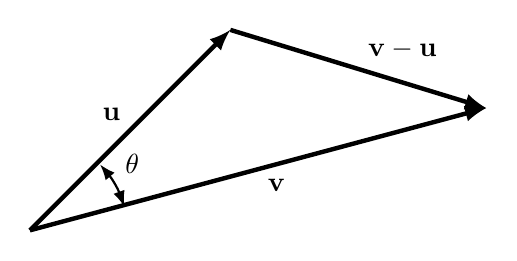
\begin{tikzpicture}[scale=1.2]  % 放大图形以更好地展示
                % 定义向量长度和角度
                \pgfmathsetmacro{\ru}{3} % 向量u长度
                \pgfmathsetmacro{\rv}{5} % 向量v长度
                \pgfmathsetmacro{\alpha}{15} % 向量v与横轴夹角 ψ
                \pgfmathsetmacro{\delta}{30} % 向量v和u的夹角 θ

                % 计算坐标
                \pgfmathsetmacro{\xv}{\rv * cos(\alpha)}
                \pgfmathsetmacro{\yv}{\rv * sin(\alpha)}
                \pgfmathsetmacro{\xu}{\ru * cos(\alpha + \delta)}
                \pgfmathsetmacro{\yu}{\ru * sin(\alpha + \delta)}

                % 绘制第一个向量v
                \draw[->,>=latex, ultra thick, black] (0, 0) -- (\xv, \yv);

                % 绘制第二个向量u
                \draw[->,>=latex, ultra thick, black] (0, 0) -- (\xu, \yu);
                % 绘制第三个向量v-u
                \draw[->,>=latex, ultra thick, black] (\xu, \yu) -- (\xv, \yv);

                % 标注角度 θ
                \draw[<->,thick,black,{Latex[length=2mm]}-{Latex[length=2mm]}] (1cm,0.25cm) arc [start angle=\alpha, end angle=\alpha+\delta, radius=1cm] node[midway, above right] {$\theta$};

                % 标注向量长度
                \node at (\xu/2, \yu/2) [above left] {$\mathbf{u}$};
                \node at (\xv/2, \yv/2) [below right] {$\mathbf{v}$};
                \node at (\xu/2+\xv/2, \yu/2+\yv/2) [above right] {$\mathbf{v-u}$};
            \end{tikzpicture}
            \end{center}
            \caption{The lengths of the sides of the triangle are given by the magnitudes of the vectors that form the triangle.}
        \end{figure}
        Recall from trigonometry that the law of cosines describes the relationship among the side lengths of the triangle and the angle $\theta$. Applying the law of cosines here gives
        $$\|\mathbf{v-u}\|^{2}=\|\mathbf{v}\|^{2}+\|\mathbf{u}\|^{2}-2\|\mathbf{u}\|\|\mathbf{v}\|cos\theta$$.
        The dot product provides a way to rewrite the left side of Equation:
        \begin{align}
            \|\mathbf{v-u}\|^{2}&=(\mathbf{v-u})\cdot(\mathbf{v-u})\\
                                &=(\mathbf{v-u})\cdot\mathbf{v}-(\mathbf{v-u})\cdot\mathbf{u}\\
                                &=\mathbf{v}\cdot\mathbf{v}-\mathbf{u}\cdot\mathbf{v}-\mathbf{v}\cdot\mathbf{u}+\mathbf{u}\cdot\mathbf{u}\\
                                &=\mathbf{v}\cdot\mathbf{v}-\mathbf{u}\cdot\mathbf{v}-\mathbf{u}\cdot\mathbf{v}+\mathbf{u}\cdot\mathbf{u}\\
                                &=\|\mathbf{v}\|^{2}-2\mathbf{u}\cdot\mathbf{v}+\|\mathbf{u}\|^{2}
        \end{align}
        Substituting into the law of cosines yields
        \begin{align}
            \|\mathbf{v-u}\|^{2}&=\|\mathbf{u}\|^{2}+\|\mathbf{v}\|^{2}-2\|\mathbf{u}\|\|\mathbf{v}\|\mathbf{cos\theta}\\            \|\mathbf{v}\|^{2}-2\mathbf{u}\cdot\mathbf{v}+\|\mathbf{u}\|^{2}&=\|\mathbf{u}\|^{2}+\|\mathbf{v}\|^{2}-2\|\mathbf{u}\|\|\mathbf{v}\|\mathbf{cos\theta}\\
            -2\mathbf{u}\cdot\mathbf{v}&=-2\|\mathbf{u}\|\|\mathbf{v}\|\mathbf{cos\theta}\\
            \mathbf{u}\cdot\mathbf{v}&=\|\mathbf{u}\|\|\mathbf{v}\|\mathbf{cos\theta}
        \end{align}
    }

    \defn{Orthogonal Vector}{
        If the inner product between two nonzero vectors is zero, we say that the vectors are orthogonal.
        $$\langle \mathbf{u}\mathbf{v} \rangle=\mathbf{u} \cdot \mathbf{v}=\mathbf{u}^{\mathbf{T}}\mathbf{v}=\mathbf{0}$$
    }

    \defn{The norm of a vector}{
        $$\|\mathbf{u}\|=(\mathbf{u}^{\mathbf{T}}\mathbf{u})^{1/2}=(u^2_{1}+u^2_{2}+\cdots+u^2_{n})^{1/2}$$
    }

    \defn{Normalized Vector}{
        If the norm of a vector is equal to one, we say that the vector is normalized.
        $$\|\mathbf{u}\|=1$$
    }

    \defn{Orthonormal Vector}{
        If a set of vectors are mutually orthogonal and normalized, we say that these vectors are orthonormal.
         $$\langle \mathbf{u}_{i}\mathbf{u}_{j} \rangle=(\mathbf{u}_{i})^{\mathbf{T}}\mathbf{u}_{j}=0\ (i \neq j)\ and\ \|\mathbf{u}_{n}\|=1$$
    }

    \defn{Outer product}{
        \begin{align}
            \mathbf{u} \otimes \mathbf{v}&=\mathbf{u}\mathbf{v}^{\mathbf{T}}\\
                &=
                \begin{pmatrix}
                    u_{1}\\
                    u_{2}\\
                    \vdots\\
                    u_{n}
                \end{pmatrix}
                \begin{pmatrix}
                    v_{1} & v_{2} & \cdots & v_{n}
                \end{pmatrix}\\
                &=
                \begin{pmatrix}
                    u_{1}v_{1} & u_{1}v_{2} & \cdots & u_{1}v_{n}\\
                    u_{2}v_{1} & v_{2}v_{2} & \cdots & u_{2}v_{n}\\
                    \vdots     & \vdots     & \ddots & \vdots\\
                    u_{n}v_{1} & v_{n}v_{2} & \cdots & u_{n}v_{n}
                \end{pmatrix}
        \end{align}
        Notice that every column is a multiple of the single vector $\mathbf{u}$, and every row is a multiple of the single vector $\mathbf{v}^{\mathbf{T}}$.
    }

    \defn{The trace of a square matrix}{
        The trace of a square matrix $\mathbf{A}$, denoted as $\operatorname{Tr}\mathbf{A}$, is the sum of the diagonal elements of $\mathbf{A}$.

    }

    \cor{
         $\operatorname{Tr}(\mathbf{A}^{\mathbf{T}}\mathbf{A})$ is the sum of the squares of all the elements of $\mathbf{A}$.
    }
    \pf{
        Let $\mathbf{A}$ be an m-by-n matrix. Then
        $$\operatorname{Tr}(\mathbf{A}^{\mathbf{T}}\mathbf{A})=\sum_{j=1}^{n}(\mathbf{A}^{\mathbf{T}}\mathbf{A})_{jj}=\sum_{j=1}^{n}\sum_{i=1}^{m}(a_{ji})^{\mathbf{T}}a_{ij}=\sum_{j=1}^{n}\sum_{i=1}^{m}(a_{ij})^2$$
        which is the sum of the squares of all the elements of A.
    }
}

\section{Inverse matrix}{
    \textbf{Square matrices} may have inverses, i.e. some matrices don't have inverses.
    \defn{Inverse matrix}{
        When a \textbf{square matrix} $\mathbf{A}$ has an inverse, we say it is invertible (or nonsingular) and denote its inverse by $\mathbf{A}^{-1}$. The inverse matrix satisfies
        $$\mathbf{A}\mathbf{A}^{-1} = \mathbf{A}^{-1}\mathbf{A} = \mathbf{I}$$
        If a \textbf{square matrix} $\mathbf{A}$ has no inverse, we say $\mathbf{A}$ is singular or non-invertible.
    }

    \cor{
        If a \textbf{square matrix} $\mathbf{A}$ is invertible, then
        $$(\mathbf{A}^{-1})^{-1}=\mathbf{A}$$
    }

    \cor{
        If $\mathbf{A}$ and $\mathbf{B}$ are invertible matrices, then
        $$(\mathbf{A}\mathbf{B})^{-1}=\mathbf{B}^{-1}\mathbf{A}^{-1}$$
    }
    \pf{
        From the definition of an inverse,
        $$(\mathbf{A}\mathbf{B})^{-1}(\mathbf{A}\mathbf{B})=\mathbf{I}$$
        $$(\mathbf{A}\mathbf{B})(\mathbf{A}\mathbf{B})^{-1}=\mathbf{I}$$
        Either multiply on the right by $\mathbf{B}^{-1}$, and then by $\mathbf{A}^{-1}$, or multiply on the left by $\mathbf{A}^{-1}$, and then by $\mathbf{B}^{-1}$, to obtain
        $$(\mathbf{A}\mathbf{B})^{-1}=\mathbf{B}^{-1}\mathbf{A}^{-1}$$
    }

    \cor{
         if $\mathbf{A}$ is invertible, then so is $\mathbf{A}^{\mathbf{T}}$, and
         $$(\mathbf{A}^{\mathbf{T}})^{-1} = (\mathbf{A}^{-1})^{\mathbf{T}}$$
    }
    \pf{
        We assume that A is invertible so that
        $$\mathbf{A}\mathbf{A}^{-1}=\mathbf{I}\ and\ \mathbf{A}^{-1}\mathbf{A}=\mathbf{I}$$
        Taking the transpose of both sides of these two equations, using both $\mathbf{I}^{\mathbf{T}}=\mathbf{I}$ and $(\mathbf{A}\mathbf{B})^{\mathbf{T}} =\mathbf{B}^{\mathbf{T}}\mathbf{A}^{\mathbf{T}}$, we obtain
        $$(\mathbf{A}\mathbf{A}^{-1})^{\mathbf{T}}=(\mathbf{A}^{-1})^{\mathbf{T}}\mathbf{A}^{\mathbf{T}}=\mathbf{I}^{\mathbf{T}}=\mathbf{I}\ and\ (\mathbf{A}^{-1}\mathbf{A})^{\mathbf{T}}=\mathbf{A}^{\mathbf{T}}(\mathbf{A}^{-1})^{\mathbf{T}}=\mathbf{I}^{\mathbf{T}}=\mathbf{I}$$.
        Therefore, since we have found that $(\mathbf{A}^{-1})^{\mathbf{T}}\mathbf{A}^{\mathbf{T}}=\mathbf{I}$ and $\mathbf{A}^{\mathbf{T}}(\mathbf{A}^{-1})^{\mathbf{T}}=\mathbf{I}$,
        we conclude that $\mathbf{A}^{\mathbf{T}}$ is invertible and that $(\mathbf{A}^{\mathbf{T}})^{-1}=(\mathbf{A}^{-1})^{\mathbf{T}}$.
    }

    \defn{The determinant of the two-by-two matrix}{
        $\mathbf{A}$ is a two-by-two matrix, i.e.
        $\mathbf{A}=
            \begin{pmatrix}
                a & b\\
                c & d
            \end{pmatrix}$
        , then the determinant of $\mathbf{A}$ is
        $$\det\mathbf{A}=\det
            \begin{pmatrix}
                a & b\\
                c & d
            \end{pmatrix}
            =ad-bc$$
        Evidently, a two-by-two matrix A is invertible only if $\det{\mathbf{A}} \neq \mathbf{0}$.
        $$\mathbf{A}^{-1}=
            \frac{1}{\det\mathbf{A}}
                \begin{pmatrix}
                    d & -b\\
                    -c & a
                \end{pmatrix}
            =
            \frac{1}{ad-bc}
                \begin{pmatrix}
                    d & -b\\
                    -c & a
                \end{pmatrix}$$
        Notice that the inverse of a two-by-two matrix, in words, is found by switching the diagonal elements of the matrix, negating the off-diagonal elements, and dividing by the determinant.
    }
    \pf{
        Let two-by-two matrix
        $\mathbf{M}=
            \begin{pmatrix}
                a & b\\
                c & d
            \end{pmatrix}$
        , and the inverse matrix is
        $\begin{pmatrix}
            x_{1} & x_{2}\\
            y_{1} & y_{2}
        \end{pmatrix}$
        . Then
        $$\begin{pmatrix}
            a & b\\
            c & d
        \end{pmatrix}
        \begin{pmatrix}
            x_{1} & x_{2}\\
            y_{1} & y_{2}
        \end{pmatrix}
        =
        \begin{pmatrix}
            1 & 0\\
            0 & 1
        \end{pmatrix}$$
        To solve, we can eliminate $y_{1}$ and $y_{2}$ using the two homogeneous equations, and find $x_{1}$ and $x_{2}$ using the two inhomogeneous equations. The solution for the inverse matrix is found to be
        $$\begin{pmatrix}
            a & b\\
            c & d
        \end{pmatrix}^{-1}
        =\frac{1}{ad-bc}
        \begin{pmatrix}
            d & -b\\
            -c & a
        \end{pmatrix}$$
        The term $ad-bc$ is just the definition of the determinant of the two-by-two matrix.
    }

    \cor{
        An n-by-n matrix is invertible if and only if its determinant is nonzero.
        \[\det(\mathbf{A})=\sum_{j=1}^n(-1)^{i+j}a_{ij}\det(\mathbf{A}_{ij})\] where $\mathbf{A}_{ij}$ is the (n-1)×(n-1) submatrix obtained by removing the i-th row and j-th column.
    }

    \cor{
        if a matrix is invertible, then its inverse is unique.
    }
    \pf{
        Let $\mathbf{A}$ be an invertible matrix, and suppose $\mathbf{B}$ and $\mathbf{C}$ are its inverse. To prove that $\mathbf{B}=\mathbf{C}$, we write
        $$\mathbf{B}=\mathbf{B}\mathbf{I}=\mathbf{B}(\mathbf{A}\mathbf{C})=(\mathbf{B}\mathbf{A})\mathbf{C}=\mathbf{I}\mathbf{C}=\mathbf{C}$$
    }

}

\section{Orthogonal matrix}{
    \defn{Orthogonal matrix}{
        A square matrix Q with real entries that satisfies
        $$\mathbf{Q}^{-1}=\mathbf{Q}^{\mathbf{T}}$$
        is called an orthogonal matrix. Another way to write this definition is
        $$\mathbf{Q}\mathbf{Q}^{\mathbf{T}}=\mathbf{I}\ and\ \mathbf{Q}^{\mathbf{T}}\mathbf{Q}=\mathbf{I}$$

        Therefore, an equivalent definition of an orthogonal matrix is a square matrix with real entries whose columns (and also rows) form a set of orthonormal vectors.

        There is a third equivalent definition of an orthogonal matrix. Let $\mathbf{Q}$ be an n-by-n orthogonal matrix, and let $\mathbf{x}$ be an n-by-one column vector. Then the length squared of the vector $\mathbf{Qx}$ is given by
        $$\|\mathbf{Qx}\|^2=\mathbf{(Qx)^T(Qx)}=\mathbf{x^TQ^TQx}=\mathbf{x^TIx}=\mathbf{x^Tx}=\|\mathbf{x}\|^2$$
        The length of $\mathbf{Qx}$ is therefore equal to the length of $\mathbf{x}$, and we say that an orthogonal matrix is a matrix that preserves lengths.
    }
}

\section{Rotation matrices}{
    \cor{
        A matrix that rotates a vector in space doesn’t change the vector’s length and so should be an orthogonal matrix.
        $$\mathbf{R}_{\theta}=
            \begin{pmatrix}
                cos{\theta} & -sin{\theta}\\
                sin{\theta} & cos{\theta}
            \end{pmatrix}$$
        $$(\mathbf{R}_{\theta})^{\mathbf{-1}}=(\mathbf{R}_{\theta})^{\mathbf{T}}$$
        $$(\mathbf{R}_{\theta})^{\mathbf{T}}\mathbf{R}_{\theta}=\mathbf{I}$$
        $$\mathbf{R}_{\theta}(\mathbf{R}_{\theta})^{\mathbf{T}}=\mathbf{I}$$
        $$\|\mathbf{R}_{\theta}\mathbf{x}\|^2=(\mathbf{R}_{\theta}\mathbf{x})^{\mathbf{T}}(\mathbf{R}_{\theta}\mathbf{x})=\mathbf{x}^{\mathbf{T}}(\mathbf{R}_{\theta})^{\mathbf{T}}\mathbf{R}_{\theta}\mathbf{x}=\mathbf{x}^{\mathbf{T}}\mathbf{I}\mathbf{x}=\mathbf{x}^{\mathbf{T}}\mathbf{x}=\|\mathbf{x}\|^2$$
    }
    \pf{
        \begin{figure}[H]
            \begin{center}
            \begin{tikzpicture}[scale=1.2]  % 放大图形以更好地展示
                % 定义向量长度和角度
                \pgfmathsetmacro{\r}{5} % 向量长度
                \pgfmathsetmacro{\alpha}{30} % 向量 (x,y) 与横轴夹角 ψ
                \pgfmathsetmacro{\delta}{15} % 向量 (x,y) 和 (x',y') 的夹角 θ

                % 计算坐标
                \pgfmathsetmacro{\x}{\r * cos(\alpha)}
                \pgfmathsetmacro{\y}{\r * sin(\alpha)}
                \pgfmathsetmacro{\xp}{\r * cos(\alpha + \delta)}
                \pgfmathsetmacro{\yp}{\r * sin(\alpha + \delta)}

                % 绘制x轴和y轴
                \draw[->] (-1, 0) -- (5, 0) node[right] {};
                \draw[->] (0, -1) -- (0, 5) node[above] {};

                % 绘制第一个向量 (x, y)
                \draw[->, thick, black] (0, 0) -- (\x, \y) node[above left] {$(x, y)$};
                % 绘制第一个向量在轴上的投影
                \draw[dashed] (\x, \y) -- (\x, 0) node[below] {$x$};
                \draw[dashed] (\x, \y) -- (0, \y) node[left] {$y$};

                % 绘制第二个向量 (x', y')
                \draw[->, thick, black] (0, 0) -- (\xp, \yp) node[above left] {$(x', y')$};
                % 绘制第二个向量在轴上的投影
                \draw[dashed] (\xp, \yp) -- (\xp, 0) node[below] {$x'$};
                \draw[dashed] (\xp, \yp) -- (0, \yp) node[left] {$y'$};

                % 标注角度 ψ 和 θ
                \draw[<->,thick,black,{Latex[length=2mm]}-{Latex[length=2mm]}] (1cm,0cm) arc [start angle=0, end angle=\alpha, radius=1cm] node[midway, right]{$\psi$};
                \draw[<->,thick,black,{Latex[length=2mm]}-{Latex[length=2mm]}] (1.75cm,1cm) arc [start angle=\alpha, end angle=\alpha+\delta, radius=2cm] node[midway, above right] {$\theta$};

                % 标注向量长度
                \node at (\x/2, \y/2) [below right] {$r$};
                \node at (\xp/2, \yp/2) [above left] {$r$};
            \end{tikzpicture}
            \end{center}
            \caption{Rotating a vector in the x-y plane.}
        \end{figure}
        Consider the two-by-two rotation matrix that rotates a vector counterclockwise through an angle $\theta$ in the x-y plane, shown above. Since $\mathbf{x}=\mathbf{r}cos{\psi}$ and $\mathbf{y}=\mathbf{r}sin{\psi}$, trigonometry and the addition formula for cosine and sine results in
        \begin{align}
            \mathbf{x}^{'}&=\mathbf{r}cos({\theta}+{\psi})\\
                         &=\mathbf{r}(cos{\theta}cos{\psi}-sin{\theta}sin{\psi})\\
                         &=\mathbf{x}cos{\theta}-\mathbf{y}sin{\theta}
        \end{align}
        \begin{align}
            \mathbf{y}^{'}&=\mathbf{r}sin({\theta}+{\psi})\\
                         &=\mathbf{r}(sin{\theta}cos{\psi}+cos{\theta}sin{\psi})\\
                         &=\mathbf{x}sin{\theta}+\mathbf{y}cos{\theta}
        \end{align}
        Writing the equations for $\mathbf{x}^{'}$ and $\mathbf{y}^{'}$ in matrix form, we have
        $$\begin{pmatrix}
            \mathbf{x}^{'}\\
            \mathbf{y}^{'}
        \end{pmatrix}
        =
        \begin{pmatrix}
            cos{\theta} & -sin{\theta}\\
            sin{\theta} & cos{\theta}
        \end{pmatrix}
        \begin{pmatrix}
            \mathbf{x}\\
            \mathbf{y}
        \end{pmatrix}$$
        The above two-by-two matrix is a rotation matrix and we will denote it by $\mathbf{R}_{\theta}$. Observe that the rows and columns of $\mathbf{R}_{\theta}$ are orthonormal and that the inverse of $\mathbf{R}_{\theta}$ is just its transpose. The inverse of $\mathbf{R}_{\theta}$ rotates a vector by $-\theta$.
    }

    \cor{
        $$\mathbf{R}_{(-\theta)}=(\mathbf{R}_{\theta})^{-1}$$
    }
    \pf{
        Since $\mathbf{R}_{\theta}=
            \begin{pmatrix}
                cos{\theta} & -sin{\theta}\\
                sin{\theta} & cos{\theta}
            \end{pmatrix}$
        and $(\mathbf{R}_{\theta})^{\mathbf{-1}}=(\mathbf{R}_{\theta})^{\mathbf{T}}$, then
        \begin{align}
            \mathbf{R}_{(-\theta)}&=
                \begin{pmatrix}
                    cos{(-\theta)} & -sin{(-\theta)}\\
                    sin{(-\theta)} & cos{(-\theta)}
                \end{pmatrix}\\
                &=
                \begin{pmatrix}
                    cos{\theta} & sin{\theta}\\
                    -sin{\theta} & cos{\theta}
                \end{pmatrix}\\
                &=(\mathbf{R}_{\theta})^{\mathbf{T}}\\
                &=(\mathbf{R}_{\theta})^{-1}
        \end{align}
    }
}

\section{Permutation matrices}{
    \defn{Permutation matrix}{
        A permutation matrix is a \textbf{square matrix} obtained by permuting the rows or columns of an \textbf{identity matrix}.\\
        A permutation matrix is a \textbf{square matrix} that has exactly one entry of 1 in each row and each column with all other entries 0.


    }

    \cor{
        A permutation matrix, when multiplying on the left, permutes the rows of a matrix, and when multiplying on the right, permutes the columns. Clearly, permuting the rows of a column vector will not change its length.
    }

    \cor{
        The identity matrix is a permutation matrix.
    }

    \cor{
        A permutation matrix is orthogonal.
    }

    \cor{
        $$\mathbf{PA=(PI)A}$$
        where P is a permutation matrix and PI is the identity matrix with permuted rows.
    }

    \cor{
        Six three-by-three permutation matrices:
        $$\mathbf{P}_{123}=
            \begin{pmatrix}
                1 & 0 & 0\\
                0 & 1 & 0\\
                0 & 0 & 1
            \end{pmatrix}
        ,\
        \mathbf{P}_{132}=
            \begin{pmatrix}
                1 & 0 & 0\\
                0 & 0 & 1\\
                0 & 1 & 0
            \end{pmatrix}
        ,\
        \mathbf{P}_{213}=
            \begin{pmatrix}
                0 & 1 & 0\\
                1 & 0 & 0\\
                0 & 0 & 1
            \end{pmatrix}
        ,$$
        $$\mathbf{P}_{231}=
            \begin{pmatrix}
                0 & 0 & 1\\
                1 & 0 & 0\\
                0 & 1 & 0
            \end{pmatrix}
        ,\
        \mathbf{P}_{312}=
            \begin{pmatrix}
                0 & 1 & 0\\
                0 & 0 & 1\\
                1 & 0 & 0
            \end{pmatrix}
        ,\
        \mathbf{P}_{321}=
            \begin{pmatrix}
                0 & 0 & 1\\
                0 & 1 & 0\\
                1 & 0 & 0
            \end{pmatrix}
        $$
        The inverses of all three-by-three permutation matrices(Since they are all orthogonal matrices, $\mathbf{P}^{-1}=\mathbf{P}^{\mathbf{T}}$):
        $$(\mathbf{P}_{123})^{-1}=(\mathbf{P}_{123})^{\mathbf{T}}
            =
            \begin{pmatrix}
                1 & 0 & 0\\
                0 & 1 & 0\\
                0 & 0 & 1
            \end{pmatrix}^{\mathbf{T}}
            =
            \begin{pmatrix}
                1 & 0 & 0\\
                0 & 1 & 0\\
                0 & 0 & 1
            \end{pmatrix}
            =
            \mathbf{P}_{123}$$
        $$(\mathbf{P}_{132})^{-1}=(\mathbf{P}_{132})^{\mathbf{T}}
            =
            \begin{pmatrix}
                1 & 0 & 0\\
                0 & 0 & 1\\
                0 & 1 & 0
            \end{pmatrix}^{\mathbf{T}}
            =
            \begin{pmatrix}
                1 & 0 & 0\\
                0 & 0 & 1\\
                0 & 1 & 0
            \end{pmatrix}
            =
            \mathbf{P}_{132}$$
        $$(\mathbf{P}_{213})^{-1}=(\mathbf{P}_{213})^{\mathbf{T}}
            =
            \begin{pmatrix}
                0 & 1 & 0\\
                1 & 0 & 0\\
                0 & 0 & 1
            \end{pmatrix}^{\mathbf{T}}
            =
            \begin{pmatrix}
                0 & 1 & 0\\
                1 & 0 & 0\\
                0 & 0 & 1
            \end{pmatrix}
            =
            \mathbf{P}_{213}$$
        $$(\mathbf{P}_{231})^{-1}=(\mathbf{P}_{231})^{\mathbf{T}}
            =
            \begin{pmatrix}
                0 & 0 & 1\\
                1 & 0 & 0\\
                0 & 1 & 0
            \end{pmatrix}^{\mathbf{T}}
            =
            \begin{pmatrix}
                0 & 1 & 0\\
                0 & 0 & 1\\
                1 & 0 & 0
            \end{pmatrix}
            =
            \mathbf{P}_{312}$$
        $$(\mathbf{P}_{312})^{-1}=(\mathbf{P}_{312})^{\mathbf{T}}
            =
            \begin{pmatrix}
                0 & 1 & 0\\
                0 & 0 & 1\\
                1 & 0 & 0
            \end{pmatrix}^{\mathbf{T}}
            =
            \begin{pmatrix}
                0 & 0 & 1\\
                1 & 0 & 0\\
                0 & 1 & 0
            \end{pmatrix}
            =
            \mathbf{P}_{231}$$
        $$(\mathbf{P}_{321})^{-1}=(\mathbf{P}_{321})^{\mathbf{T}}
            =
            \begin{pmatrix}
                0 & 0 & 1\\
                0 & 1 & 0\\
                1 & 0 & 0
            \end{pmatrix}^{\mathbf{T}}
            =
            \begin{pmatrix}
                0 & 0 & 1\\
                0 & 1 & 0\\
                1 & 0 & 0
            \end{pmatrix}
            =
            \mathbf{P}_{321}$$
    }
}

\chapter{Systems of Linear Equations}

\section{Gaussian elimination}{
    \defn{Gaussian Elimination}{
        Gaussian elimination is a method for solving matrix equations of the form
        $$\mathbf{A}\mathbf{x}=\mathbf{b}$$
        To perform Gaussian elimination starting with the system of equations
        \begin{equation}
            \begin{bmatrix}
                a_{11} & a_{12} & \cdots & a_{1n}\\
                a_{21} & a_{22} & \cdots & a_{2n}\\
                \vdots & \vdots & \ddots & \vdots\\
                a_{n1} & a_{n2} & \cdots & a_{nn}
            \end{bmatrix}
            \begin{bmatrix}
                x_{1}\\
                x_{2}\\
                \vdots\\
                x_{n}
            \end{bmatrix}
            =
            \begin{bmatrix}
                b_{1}\\
                b_{2}\\
                \vdots\\
                b_{n}
            \end{bmatrix}
        \end{equation}
        compose the "augmented matrix equation"
        \begin{equation}
            \begin{bmatrix}
                \begin{array}{cccc|c}
                    a_{11} & a_{12} & \cdots & a_{1n} & b_{1}\\
                    a_{21} & a_{22} & \cdots & a_{2n} & b_{2}\\
                    \vdots & \vdots & \ddots & \vdots & \vdots\\
                    a_{n1} & a_{n2} & \cdots & a_{nn} & b_{n}
                \end{array}
            \end{bmatrix}
            \begin{bmatrix}
                x_{1}\\
                x_{2}\\
                \vdots\\
                x_{n}
            \end{bmatrix}
        \end{equation}
        Here, the column vector in the variables $\mathbf{x}$ is carried along for labeling the matrix rows. Now, perform elementary row operations to put the augmented matrix into the upper triangular form
        \begin{equation}
            \begin{bmatrix}
                \begin{array}{cccc|c}
                    a_{11}^{'} & a_{12}^{'} & \cdots & a_{1n}^{'} & b_{1}^{'}\\
                    0          & a_{22}^{'} & \cdots & a_{2n}^{'} & b_{2}^{'}\\
                    \vdots     & \vdots     & \ddots & \vdots     & \vdots\\
                    0          & 0          & \cdots & a_{nn}^{'} & b_{n}^{'}
                \end{array}
            \end{bmatrix}
        \end{equation}
    }

    \cor{
        Solve the equation of the kth row for $\mathbf{x}_{k}$, then substitute back into the equation of the (k-1)st row to obtain a solution for $\mathbf{x}_{k-1}$, etc., according to the formula
        $$x_{i}=\frac{1}{a_{ii}^{'}}\left(b_{i}^{'}-\sum_{j=i+1}^{n}a_{ij}^{'}x_{j}\right)$$
    }

    \defn{pivot}{
        When performing Gaussian elimination, the matrix element that is used during the elimination procedure is called the pivot.
    }

    \cor{
         Gaussian elimination can be used on any rectangular matrix $\mathbf{A_{m \times n}}$.
    }
}

\section{Reduced row echelon form}{
    \defn{Reduced row echelon form}{
        A matrix is said to be in reduced row echelon form if the first nonzero entry in every row is a one, all the entries below and above this one are zero, and any zero rows occur at the bottom of the matrix.
    }

    \cor{
        The row elimination procedure of Gaussian elimination can be continued to bring a matrix to reduced row echelon form. We notate the reduced row echelon form of a matrix $\mathbf{A}$ as $\operatorname{rref}(\mathbf{A})$.
    }

    \cor{
        The matrix in reduced row echelon form has the following characteristics:\\
        1. All zero rows are at the bottom of the matrix\\
        2. The leading entry of each nonzero row after the first occurs to the right of the leading entry of the previous row.\\
        3. The leading entry in any nonzero row is 1.\\
        4. All entries in the column above and below a leading 1 are zero.
    }

    \defn{Pivot row}{
        Each nonzero row of $\operatorname{rref}(\mathbf{A})$ is called a pivot row.
    }

    \defn{Pivot}{
        The first nonzero in each row of $\operatorname{rref}(\mathbf{A})$ is called a pivot.
    }
    \defn{Pivot column}{
        Each column that contains a pivot in $\operatorname{rref}(\mathbf{A})$ is called a pivot column.
    }

    \cor{
        The reduced row echelon form of a matrix A is unique.
    }
    \todo[color=yellow, inline]{
        How to prove it?
    }

    \cor{
         if $\mathbf{A}$ is a square invertible matrix, then $\operatorname{rref}(\mathbf{A})$ is the identity matrix.
    }
    \todo[color=yellow, inline]{
        How to prove it?
    }
}

\section{Computing inverses}{
    \defn{Finding the inverse of a matrix}{
        If $\mathbf{A}$ is an $n \times n$ \textbf{square matrix}, then one can use row reduction to compute its inverse matrix, if it exists. First, the $n \times n$ identity matrix is augmented to the right of $\mathbf{A}$, forming an $n \times 2n$ block matrix $[\mathbf{A \mid I}]$. Now through application of elementary row operations, find the reduced echelon form of this $n \times 2n$ matrix. The matrix $\mathbf{A}$ is invertible if and only if the left block can be reduced to the identity matrix $\mathbf{I}$; in this case the right block of the final matrix is $\mathbf{A}^{-1}$. If the algorithm is unable to reduce the left block to $\mathbf{I}$, then $\mathbf{A}$ is not invertible.
        \begin{equation}
            [\mathbf{A \mid I}]=
                \begin{bmatrix}
                    \begin{array}{cccc|cccc}
                        a_{11} & a_{12} & \cdots & a_{1n} & 1      & 0      & \cdots & 0\\
                        a_{21} & a_{22} & \cdots & a_{2n} & 0      & 1      & \cdots & 0\\
                        \vdots & \vdots & \ddots & \vdots & \vdots & \vdots & \ddots & \vdots\\
                        a_{n1} & a_{n2} & \cdots & a_{nn} & 0      & 0      & \cdots & 1
                    \end{array}
                \end{bmatrix}\\
            \xrightarrow{}
            [\mathbf{I \mid B}]=
                \begin{bmatrix}
                    \begin{array}{cccc|cccc}
                        1      & 0      & \cdots & 0      & b_{11} & b_{12} & \cdots & b_{1n}\\
                        0      & 1      & \cdots & 0      & b_{21} & b_{22} & \cdots & b_{2n}\\
                        \vdots & \vdots & \ddots & \vdots & \vdots & \vdots & \ddots & \vdots\\
                        0      & 0      & \cdots & 1      & b_{n1} & b_{n2} & \cdots & b_{nn}
                    \end{array}
                \end{bmatrix}
        \end{equation}
        On the left, that $\mathbf{BA=I}$, therefore $\mathbf{B=A^{-1}}$. On the right, we kept a record of $\mathbf{BI=B}$. So
        \begin{equation}
            \mathbf{A^{-1}}=
                \begin{bmatrix}
                        b_{11} & b_{12} & \cdots & b_{1n}\\
                        b_{21} & b_{22} & \cdots & b_{2n}\\
                        \vdots & \vdots & \ddots & \vdots\\
                        b_{n1} & b_{n2} & \cdots & b_{nn}
                \end{bmatrix}
        \end{equation}
    }
}

\section{Elementary matrices}{
    \defn{Elementary matrix}{
        An elementary matrix $\mathbf{E}$ is a \textbf{square matrix} obtained from the application of a single elementary row operation to the \textbf{identity matrix}.
    }

    \cor{
        The row reduction algorithm of Gaussian elimination can be implemented by multiplying elementary matrices.
    }

    \ex{
        $$\mathbf{M_{3}M_{2}M_{1}A=U}$$
        where U is an upper triangular matrix.
    }
}

\section{LU decomposition}{
    \defn{LU decomposition}{
        A procedure for decomposing an matrix $\mathbf{A}$ into a product of a lower triangular matrix $\mathbf{L}$ and an upper triangular matrix $\mathbf{U}$,
        $$\mathbf{LU=A}$$
    }

    \ex{
        If $\mathbf{M_{3}M_{2}M_{1}A=U}$, where U is an upper triangular matrix, then
        $$\mathbf{L=M_{1}^{-1}M_{2}^{-1}M_{3}^{-1}}$$
    }
}

\section{Solving (LU)x = b}{
    \defn{Solving (LU)x = b}{
        The $\mathbf{LU}$ decomposition is useful when one needs to solve
        $$\mathbf{Ax=b}$$
        for $\mathbf{x}$ when the matrix $\mathbf{A}$ is fixed and there are many different $\mathbf{b}$’s. First one determines $\mathbf{L}$ and $\mathbf{U}$ using Gaussian elimination. Then one writes
        $$\mathbf{(LU)x=L(Ux)=b}$$
        We let
        $$\mathbf{y=Ux}$$
        and first solve
        $$\mathbf{Ly=b}$$
        for $\mathbf{y}$. This can be done by forward substitution
        \ex{
            $$y_{1}=\frac{b_{1}}{l_{11}}$$
            $$y_{i}=\frac{1}{l_{ii}}\left(b_{i}-\sum_{j=1}^{i-1}l_{ij}y_{j}\right)$$
            for square matrix A with $i=2,\ldots,n\text{ and }l_{ii}\neq0$.
        }\\
        Then solve
        $$\mathbf{Ux=y}$$
        for $\mathbf{x}$. This can be done by back substitution
        \ex{
            $$x_{n}=\frac{y_{n}}{u_{nn}}$$
            $$x_{i}=\frac{1}{u_{ii}}\left(y_{i}-\sum_{j=i+1}^{n}u_{ij}x_{j}\right)$$
            for square matrix A $i=n-1,\ldots,1\text{ and }u_{ii}\neq0$.
        }\\
        If we count operations, we can show that solving $\mathbf{(LU)x=b}$ is a factor of n faster once $\mathbf{L}$ and $\mathbf{U}$ are in hand than solving $\mathbf{Ax=b}$ directly by Gaussian elimination.
    }
}

\chapter{Vector Spaces}

\section{Vector spaces}{
    \defn{Vector spaces}{
        A vector space consists of a set of vectors and a set of scalars. For the set of vectors and scalars to form a vector space, the set of vectors must be closed under vector addition and scalar multiplication. That is, when you multiply any two vectors in the set by real numbers and add them, the resulting vector must still be in the set.
    }

    \cor{
        A vector space V is a set that is \textbf{closed under finite vector addition and scalar multiplication}.\\
        For a general vector space, the scalars are members of a field $\mathbf{F}$, in which case $\mathbf{V}$ is called a vector space over $\mathbf{F}$.\\
        In order for $\mathbf{V}$ to be a vector space, the following conditions must hold for all elements $\mathbf{X,Y,Z} \in \mathbf{V}$ and any scalars $\mathbf{r,s} \in \mathbf{F}$:
        \begin{enumerate}
          \item \textbf{(Additive Closure)} $\mathbf{X+Y} \in \mathbf{V}$. Adding two vectors gives a vector.
          \item \textbf{(Additive Commutativity)} $\mathbf{X+Y=Y+X}$. Order of addition doesn't matter.
          \item \textbf{(Additive Associativity)} $\mathbf{(X+Y)+Z=X+(Y+Z)}$. Order of adding many vectors doesn't matter.
          \item \textbf{(Zero)} There is a special vector $\mathbf{0_{V} \in V}$ such that $\mathbf{X+0_{V}=0_{V}+X=X}$ for all $\mathbf{X}$ in $\mathbf{V}$.
          \item \textbf{(Additive Inverse)} For every $\mathbf{X \in V}$ there exists $\mathbf{-X \in V}$ such that $\mathbf{X+(-X)=0_{V}}$.
          \item \textbf{(Multiplicative Closure)} $\mathbf{rX \in V}$. Scalar times a vector is a vector.
          \item \textbf{(Distributivity)} $\mathbf{(r+s)X=rX+sX}$. Scalar multiplication distributes over addition of scalars.
          \item \textbf{(Distributivity)} $\mathbf{r(X+Y)=rX+rY}$. Scalar multiplication distributes over addition of vectors.
          \item \textbf{(Associativity)} $\mathbf{(rs)X=r(sX)}$.
          \item \textbf{(Unity)} $\mathbf{1X=X}$ for all $\mathbf{X \in V}$.
        \end{enumerate}
    }
}

\section{Linear independence}{
    \defn{Linearly independent}{
        The vectors $\mathbf{\{u_{1},u_{2},\ldots,u_{n}\}}$ are linearly independent if for any scalars $c_{1},c_{2},\ldots,c_{n}$, the equation $c_{1}\mathbf{u}_{1}+c_{2}\mathbf{u}_{2}+\ldots+c_{n}\mathbf{u}_{n}=0$ has only the solution $c_{1}=c_{2}=\ldots=c_{n}=0$. What this means is that one is unable to write any of the vectors $\mathbf{u}_{1},\mathbf{u}_{2},\ldots,\mathbf{u}_{n}$ as a linear combination of any of the other vectors.
    }

    \cor{
        place the vectors as the rows of a matrix and compute the reduced row echelon form. If the last row becomes all zeros, then the vectors are linearly dependent, and if not all zeros, then they are linearly independent
    }

    \defn{Linearly independent Vectors}{
        A list of vectors $(\mathbf{v}_{1},\ldots,\mathbf{v}_{m})$ is called linearly independent if the only solution for $a_{1},\ldots,a_{m} \in \mathbf{F}$ to the equation
        $$a_{1}\mathbf{v}_{1}+\ldots+a_{m}\mathbf{v}_{m}=0$$
        is $a_{1}=\ldots=a_{m}=0$. In other words, the zero vector can only trivially be written as a linear combination of $(\mathbf{v}_{1},\ldots,\mathbf{v}_{m})$.
    }

    \defn{Linearly dependent Vectors}{
        A list of vectors $(\mathbf{v}_{1},\ldots,\mathbf{v}_{m})$ is called linearly dependent if it is not linearly independent. That is, $(\mathbf{v}_{1},\ldots,\mathbf{v}_{m})$ is linear dependent if there exist $a_{1},\ldots,a_{m} \in \mathbf{F}$, not all zero, such that
        $$a_{1}\mathbf{v}_{1}+\ldots+a_{m}\mathbf{v}_{m}=0$$
    }
}

\section{Span, basis and dimension}{
    \defn{Span of vectors}{
        The span of the set of vectors $(\mathbf{v}_{1},\mathbf{v}_{2},\ldots,\mathbf{v}_{n})$ is the vector space consisting of all linear combinations of $\mathbf{v}_{1},\mathbf{v}_{2},\ldots,\mathbf{v}_{n}$. We say that a set of vectors spans a vector space.

        Let $\{\mathbf{v}_{1},\ldots,\mathbf{v}_{n}\} \subseteq V$, then
        $$\operatorname{span}\{\mathbf{v}_{1},\ldots,\mathbf{v}_{n}\}=\left\{\sum_{i=1}^{n}c_{i}\mathbf{v}_{i},c_{i} \in \mathbf{F}\right\}$$
    }

    \defn{Basis and Dimension}{
        The smallest set of vectors needed to span a vector space forms a basis for that vector space.\\
        The number of vectors in a basis gives the dimension of the vector space.\\
        Let $\mathbf{V}$ be a vector space.
        \begin{itemize}
            \item Then a set $\mathbf{S}$ is a basis for $\mathbf{V}$ if $\mathbf{S}$ is linearly independent and $\mathbf{V}=\operatorname{span}\{S\}$.
            \item The number of vectors in $\mathbf{S}$ is the dimension of $\mathbf{V}$.
        \end{itemize}
    }

    \cor{
        Let $\mathbf{S}=\{\mathbf{v}_{1},\ldots,\mathbf{v}_{n}\}$ be a basis for a vector space V. Then every vector $\mathbf{w} \in \mathbf{V}$ can be written uniquely as a linear combination of vectors in the basis $\mathbf{S}$:
        $$\mathbf{w}=c_{1}\mathbf{v}_{1}+\ldots+c_{n}\mathbf{v}_{n}$$
    }
}

\section{Gram-Schmidt process}{
    \defn{Gram-Schmidt process}{
        Given any basis for a vector space, we can use an algorithm called the Gram-Schmidt process to construct an orthonormal basis for that space. Let the vectors $\mathbf{v}_{1},\mathbf{v}_{2},\cdots,\mathbf{v}_{n}$ be a basis for some n-dimensional vector space. We will assume here that these vectors are column matrices, but this process also applies more generally.\\
        We will construct an orthogonal basis $\mathbf{u}_{1},\mathbf{u}_{2},\cdots,\mathbf{u}_{n}$, and then normalize each vector to obtain an orthonormal basis. First, define $\mathbf{u}_{1}=\mathbf{v}_{1}$. To find the next orthogonal basis vector, define
        $$\mathbf{u}_{2}=\mathbf{v}_{2}-\frac{(\mathbf{u}_{1}^{\mathbf{T}}\mathbf{v}_{2})\mathbf{u}_{1}}{\mathbf{u}_{1}^{\mathbf{T}}\mathbf{u}_{1}}$$.
        Observe that $\mathbf{u}_{2}$ is equal to $\mathbf{v}_{2}$ minus the component of $\mathbf{v}_{2}$ that is parallel to $\mathbf{u}_{1}$. By multiplying both sides of this equation with $\mathbf{u}_{1}^{\mathbf{T}}$, it is easy to see that $\mathbf{u}_{1}^{\mathbf{T}}\mathbf{u}_{2}=0$ so that these two vectors are orthogonal.
        The next orthogonal vector in the new basis can be found from
        $$\mathbf{u}_{3}=\mathbf{v}_{3}-\frac{(\mathbf{u}_{1}^{\mathbf{T}}\mathbf{v}_{3})\mathbf{u}_{1}}{\mathbf{u}_{1}^{\mathbf{T}}\mathbf{u}_{1}}-\frac{(\mathbf{u}_{2}^{\mathbf{T}}\mathbf{v}_{3})\mathbf{u}_{2}}{\mathbf{u}_{2}^{\mathbf{T}}\mathbf{u}_{2}}$$
        Here, $\mathbf{u}_{3}$ is equal to $\mathbf{v}_{3}$ minus the components of $\mathbf{v}_{3}$ that are parallel to $\mathbf{u}_{1}$ and $\mathbf{u}_{2}$. We can continue in this fashion to construct n orthogonal basis vectors.
        $$\mathbf{u}_{k}=\mathbf{v}_{k}-\sum_{i=1}^{k-1}\frac{(\mathbf{u}_{i}^{\mathbf{T}}\mathbf{v}_{n})\mathbf{u}_{i}}{\mathbf{u}_{i}^{\mathbf{T}}\mathbf{u}_{i}}$$
        These vectors can then be normalized via
        $$\mathbf{u}_{k}=\frac{\mathbf{u}_{k}}{(\mathbf{u}_{k}^{\mathbf{T}}\mathbf{u}_{k})^{1/2}}\text{, etc.}$$
        Since $\mathbf{u}_{k}$ is a linear combination of $\mathbf{v}_{1},\mathbf{v}_{2},\cdots,\mathbf{v}_{k}$, the vector subspace spanned by the first k basis vectors of the original vector space is the same as the subspace spanned by the first k orthonormal vectors generated through the Gram-Schmidt process. We can write this result as
        $$\operatorname{span}\{\mathbf{u}_{1},\mathbf{u}_{2},\cdots,\mathbf{u}_{k}\}=\operatorname{span}\{\mathbf{v}_{1},\mathbf{v}_{2},\cdots,\mathbf{v}_{k}\}$$
    }
}

\section{Null space}{
    \defn{Null space}{
        The null space of a matrix $\mathbf{A}$, which we denote as $\operatorname{Null}(\mathbf{A})$, is the vector space spanned by all column vectors $\mathbf{x}$ that satisfy the matrix equation
        $$\mathbf{Ax=0}$$
        For a matrix $\mathbf{A}\in\mathbb{R}^{m \times n}$, the null space of A is:
        $$\operatorname{Null}(\mathbf{A})=\{\mathbf{x}\in\mathbb{R}^{n}\mid\mathbf{Ax=0}\}$$
    }

    \cor{
        Clearly, if $\mathbf{x}$ and $\mathbf{y}$ are in the null space of $\mathbf{A}$, then so is $\mathbf{ax+by}$ so that the null space is closed under vector addition and scalar multiplication.
    }

    \cor{
        If the matrix $\mathbf{A}$ is m-by-n, then $\operatorname{Null}(\mathbf{A})$ is a vector subspace of all n-by-one column matrices.
    }

    \cor{
        If $\mathbf{A}$ is a square invertible matrix, then $\operatorname{Null}(\mathbf{A})$ consists of just the zero vector.
    }

    \defn{Basic variables}{
        The variables associated with the pivot columns are called basic variables.
    }

    \defn{Free variables}{
        The variables associated with the non-pivot columns are called free variables.
    }

    \cor{
        In general, the dimension of $\operatorname{Null}(\mathbf{A})$ is equal to the number of non-pivot columns of $\operatorname{rref}(\mathbf{A})$.
        $$\operatorname{Null}(\mathbf{A})=\operatorname{Null}(\operatorname{rref}(\mathbf{A}))$$
        $$\dim(\operatorname{Null}(\mathbf{A}))=\dim(\operatorname{Null}(\operatorname{rref}(\mathbf{A}))$$
    }

    \defn{Basis for null space}{
        To find the null space of a matrix A, follow these steps:
        \begin{enumerate}
            \item Write the system of linear equations $\mathbf{Ax=0}$.\\
                Set up the matrix equation $\mathbf{Ax=0}$, where $\mathbf{A}$ is the given matrix and $\mathbf{x}=[x_{1},x_{2},\cdots,x_{n}]^{\mathbf{T}}$ is the vector of variables.
            \item Convert the augmented matrix $[\mathbf{A\mid0}]$ to reduced row echelon form (RREF) $\operatorname{rref}([\mathbf{A \mid 0}])$.\\
                Apply row operations to transform the matrix $\mathbf{A}$ into its RREF form. The augmented matrix $[\mathbf{A \mid 0}]$ will become $[\mathbf{B \mid 0}]$, where $\mathbf{B}$ is the RREF of $\mathbf{A}$.
            \item Identify the free variables in the RREF system.\\
                The free variables are the variables that are not associated with the pivot columns in the RREF.
            \item Express the basic variables in terms of the free variables.\\
                Write the solution to the system of linear equations $\mathbf{Ax=0}$ by expressing the basic variables (the variables associated with the pivot columns) in terms of the free variables.\\
                The general solution will have the form $\mathbf{x}=c_{1}v_{1}+c_{2}v_{2}+\cdots+c_{k}v_{k}$, where $v_{1},v_{2},\cdots,v_{k}$ are the vectors corresponding to the free variables, and $c_{1},c_{2},\cdots,c_{k}$ are the free variable coefficients.
            \item The vectors $v_{1},v_{2},\cdots,v_{k}$ form a basis for the null space of A.\\
                The null space of $\mathbf{A}$ is the set of all vectors $\mathbf{x}$ that satisfy $\mathbf{Ax=0}$.\\
                The vectors $v_{1},v_{2},\cdots,v_{k}$ span the null space and represent a basis for the null space.
                $$\operatorname{Null}(\mathbf{A})=\operatorname{span}\{\mathbf{v}_{1},\ldots,\mathbf{v}_{k}\}$$
        \end{enumerate}
    }
}

\section{Application of the null space}{
    \cor{
        An under-determined system of linear equations $\mathbf{Ax=b}$ with more unknowns than equations may not have a unique solution. If $\mathbf{u}$ is the general form of a vector in the null space of $\mathbf{A}$, and $\mathbf{v}$ is any vector that satisfies $\mathbf{Av=b}$, then $\mathbf{x=u+v}$ satisfies $\mathbf{Ax=A(u+v)=Au+Av=0+b=b}$. The general solution of $\mathbf{Ax=b}$ can therefore be written as the sum of a general vector in as $\operatorname{Null}(\mathbf{A})$ and a particular vector that satisfies the under-determined system.
    }
}

\section{Column space}{
    \defn{Column space}{
        The column space of a matrix is the vector space spanned by the columns of the matrix.\\
        For a matrix $\mathbf{A}\in\mathbb{R}^{m \times n}$, the column space of A is:
        \begin{align}
            \operatorname{Col}(\mathbf{A})&=\{\mathbf{A}\mathbf{x}\mid\mathbf{x}\in\mathbb{R}^{n}\}\\
                                  &=\{c_{1}x_{1}+\cdots+c_{n}x_{n} \mid x_{1},\cdots,x_{n}\in\mathbb{R}\}
        \end{align}
        where $c_{1},\cdots,c_{n}$ are the columns of $\mathbf{A}$.\\
        Since $\mathbf{A}$ has m rows, the column space of $\mathbf{A}$ is a subspace of all m-by-one column matrices.
    }

    \cor{
        When a matrix is multiplied by a column vector, the resulting vector is in the column space of the matrix.
    }

    \cor{
        It should be self-evident that only the pivot columns of $\operatorname{rref}(\mathbf{A})$ are linearly independent, and the dimension of the column space of $\mathbf{A}$ $\operatorname{Col}(\mathbf{A})$ is therefore equal to its number of pivot columns.
        $$\operatorname{Col}(\mathbf{A})=\operatorname{Col}(\operatorname{rref}(\mathbf{A}))\text{, if }\mathbf{A}\text{ \color{red}{full rank}.}$$
        $$\dim(\operatorname{Col}(\mathbf{A}))=\dim(\operatorname{Col}(\operatorname{rref}(\mathbf{A}))$$
    }

    \defn{Basis for column space}{
        Suppose $\mathbf{A}$ is m-by-n. If columns $\{c_{j} \mid j=1,\cdots,r\}$ are the pivot columns of $\operatorname{rref}(\mathbf{A})$ then columns $\{c_{j} \mid j=1,\cdots,r\}$ of A constitute a basis for $\operatorname{Col}(\mathbf{A})$
    }

    \cor{
        Recall that the dimension of the null space is the number of non-pivot columns—equal to the number of free variables—so that the sum of the dimensions of the null space and the column space is equal to the total number of columns. A statement of this theorem is as follows. Let A be an m-by-n matrix. Then
        $$\dim(\operatorname{Col}(\mathbf{A}))+\dim(\operatorname{Null}(\mathbf{A}))=\mathbf{n}$$
    }
}

\section{Row space, left null space and rank}{
    \defn{Left null space}{
        The left null space of a matrix $\mathbf{A}\in\mathbb{R}^{m \times n}$ is the null space of its transpose, i.e.,
        \begin{align}
            \operatorname{LeftNull}(\mathbf{A})&=\operatorname{Null}(\mathbf{A}^{\mathbf{T}})\\
                                       &=\{\mathbf{y}\in\mathbb{R}^{m}\mid\mathbf{A}^{\mathbf{T}}\mathbf{y}=\mathbf{0}\}
        \end{align}
        The word "left" in this context stems from the fact that $\mathbf{A}^{\mathbf{T}}\mathbf{y}=\mathbf{0}$ is equivalent to $\mathbf{y}^{\mathbf{T}}\mathbf{A}=\mathbf{0}$ where $\mathbf{y}$ "acts" on $\mathbf{A}$ from the left.
    }

    \cor{
        $$\operatorname{LeftNull}(\mathbf{A})=\operatorname{Null}(\mathbf{A}^{\mathbf{T}})$$
        $$\operatorname{LeftNull}(\mathbf{A}^{\mathbf{T}})=\operatorname{Null}((\mathbf{A}^{\mathbf{T}})^{\mathbf{T}})=\operatorname{Null}(\mathbf{A})$$
    }

    \defn{Row space}{
        The column space of $\mathbf{A}^{\mathbf{T}}$, which are called the row space.\\
        For a matrix $\mathbf{A}\in\mathbb{R}^{m \times n}$, the row space of $\mathbf{A}$ is:
        \begin{align}
            \operatorname{Row}(\mathbf{A})&=\operatorname{Col}(\mathbf{A}^{\mathbf{T}})\\
                                  &=\{\mathbf{A}^{\mathbf{T}}\mathbf{y}\mid\mathbf{y}\in\mathbb{R}^{m}\}\\
                                  &=\{c_{1}y_{1}+\cdots+c_{n}y_{n} \mid y_{1},\cdots,y_{n}\in\mathbb{R}\}
        \end{align}
        where $c_{1},\cdots,c_{n}$ are the columns of $\mathbf{A}^{\mathbf{T}}$, i.e., the rows of $\mathbf{A}$.\\
        The row space of the m-by-n matrix A is simply the span of its rows, i.e.,
        Since $\mathbf{A}$ has n columns, the row space of $\mathbf{A}$ is a subspace of all one-by-n row matrices.
    }

    \cor{
        $$\operatorname{Row}(\mathbf{A})=\operatorname{Col}(\mathbf{A}^{\mathbf{T}})$$
        $$\operatorname{Row}(\mathbf{A}^{\mathbf{T}})=\operatorname{Col}((\mathbf{A}^{\mathbf{T}})^{\mathbf{T}})=\operatorname{Col}(\mathbf{A})$$
    }

    \defn{Basis for row space}{
        Suppose $\mathbf{A}$ is m-by-n. The pivot rows of $\operatorname{rref}(\mathbf{A})$ constitute a basis for $\operatorname{Col}(\mathbf{A}^{\mathbf{T}})$, that is $\operatorname{Row}(\mathbf{A})$.
    }

    \cor{
        If $\mathbf{A}$ is an m-by-n matrix, then the row space and the null space are subspaces of all n-by-one column matrices, and the column space and the left null space are subspaces of all m-by-one column matrices.
    }

    \cor{
        The null space consists of all vectors $\mathbf{x}$ such that $\mathbf{Ax=0}$, that is, the null space is the set of all vectors that are orthogonal to the row space of $\mathbf{A}$. We say that these two vector spaces are orthogonal.
        $$\operatorname{Null}(\mathbf{A})\perp\operatorname{Row}(\mathbf{A})$$
    }

    \cor{
        A basis for the row space of a matrix can be found from computing rref(A), and is found to be rows of rref(A) (written as column vectors) with pivot columns. The dimension of the row space of A is therefore equal to the number of pivot columns, while the dimension of the null space of A is equal to the number of nonpivot columns.
        $$\operatorname{Null}(\mathbf{A})=\operatorname{Null}(\operatorname{rref}(\mathbf{A}))$$
        $$\operatorname{Row}(\mathbf{A})=\operatorname{Row}(\operatorname{rref}(\mathbf{A}))$$
        The union of these two subspaces make up the vector space of all n-by-one matrices and we say that these subspaces are orthogonal complements of each other.
        $$\operatorname{Null}(\mathbf{A})=\operatorname{Row}(\mathbf{A})^\perp$$
        $$\operatorname{Row}(\mathbf{A})=\operatorname{Null}(\mathbf{A})^\perp$$
    }

    \defn{}{
        The nullity of a matrix $\mathbf{A}_{m \times n}$,  written $\operatorname{nullity}(\mathbf{A})$, is the dimension of the null space $\operatorname{Null}(\mathbf{A})$.
    }

    \defn{Rank}{
        The rank of a matrix $\mathbf{A}_{m \times n}$, written $\operatorname{rank}(\mathbf{A})$, is the dimension of the column space $\operatorname{Col}(\mathbf{A})$,
        which is also equal to the number of pivot columns, so that the dimensions of the column space and the row space of a matrix are equal.
        $$\operatorname{rank}(\mathbf{A})=\operatorname{rank}(\mathbf{A}^\mathbf{{T}})=\dim(\operatorname{Col}(\mathbf{A}))=\dim(\operatorname{Row}(\mathbf{A}))\leq\min\{m,n\}$$
        We call this dimension the rank of the matrix A.
    }

    \defn{Full rank}{
        When the equality $\operatorname{rank}(\mathbf{A})=\min\{m,n\}$ holds, we say that the matrix $\mathbf{A}_{m \times n}$ is of full rank.
    }

    \cor{
        \begin{align}
            \mathbf{A}_{m \times n}(m \leq n)\text{ is full row rank} &\Longleftrightarrow \text{All rows of matrix }\mathbf{A}_{m \times n}\text{ are linearly independent}\\
                                                                      &\Longleftrightarrow \operatorname{rank}(\mathbf{A}_{m \times n})=m\\
                                                                      &\Longleftrightarrow \operatorname{left\ nullity}(\mathbf{A}_{m \times n})=0\\
                                                                      &\Longleftrightarrow \mathbf{A}_{m \times n}\mathbf{A}_{m \times n}^{-1}=\mathbf{I}
        \end{align}
    }

    \cor{
        \begin{align}
            \mathbf{A}_{m \times n}(m \geq n)\text{ is full column rank} &\Longleftrightarrow \text{All columns of matrix }\mathbf{A}_{m \times n}\text{ are linearly independent}\\
                                                                         &\Longleftrightarrow \operatorname{rank}(\mathbf{A}_{m \times n})=n\\
                                                                         &\Longleftrightarrow \operatorname{nullity}(\mathbf{A}_{m \times n})=0\\
                                                                         &\Longleftrightarrow \mathbf{A}_{m \times n}^{-1}\mathbf{A}_{m \times n}=\mathbf{I}
        \end{align}
    }

    \cor{
        \begin{align}
            \mathbf{A}_{n \times n}\text{ is square full rank} &\Longleftrightarrow \text{All rows of matrix }\mathbf{A}_{n \times n}\text{ are linearly independent}\\
                                                               &\Longleftrightarrow \text{All columns of matrix }\mathbf{A}_{n \times n}\text{ are linearly independent}\\
                                                               &\Longleftrightarrow \operatorname{rank}(\mathbf{A}_{n \times n})=n\\
                                                               &\Longleftrightarrow \operatorname{nullity}(\mathbf{A}_{n \times n})=\operatorname{left\ nullity}(\mathbf{A}_{n \times n})=0\\
                                                               &\Longleftrightarrow \det(\mathbf{A}_{n \times n}) \neq n\\
                                                               &\Longleftrightarrow \mathbf{A}_{n \times n}\text{ is invertible: }\mathbf{A}_{n \times n}\mathbf{A}_{n \times n}^{-1}=\mathbf{A}_{n \times n}^{-1}\mathbf{A}_{n \times n}=\mathbf{I}
        \end{align}
    }

    \defn{Non-zero Determinant}{

    }

    \cor{
        when A is a square matrix and of full rank, then the dimension of the null space is zero and A is invertible.
    }

    \cor{
        \begin{table}[H]
            \centering
            \begin{tabular}{|c|c|c|c|}
                \hline
                \textbf{Concept} &
                \textbf{Notation} &
                \textbf{Mathematical Definition} &
                \textbf{Subspace of}\\
                \hline
                Null Space &
                $\text{Null}(\mathbf{A})=\operatorname{LeftNull}(\mathbf{A}^{\mathbf{T}})$ &
                \(
                    \begin{array}{c}
                        \text{All vectors x that}\\
                        text{ satisfy }\mathbf{A}\mathbf{x}=\mathbf{0}\\
                        \{\mathbf{x}\in\mathbb{R}^{n}\mid\mathbf{A}\mathbf{x}=\mathbf{0}\}
                    \end{array}
                \) &
                $\mathbb{R}^{n}$ (Domain of $\mathbf{A}$)\\
                \hline
                Left Null Space &
                $\operatorname{LeftNull}(\mathbf{A})=\text{Null}(\mathbf{A}^{\mathbf{T}})$ &
                \(
                    \begin{array}{c}
                        \text{All vectors y that}\\
                        \text{ satisfy }\mathbf{A}^{\mathbf{T}}\mathbf{y}=\mathbf{0}\\
                        \{\mathbf{y}\in\mathbb{R}^{m}\mid\mathbf{A}^{\mathbf{T}}\mathbf{y}=\mathbf{0}\}
                    \end{array}
                \) &
                $\mathbb{R}^{m}$ (Codomain of $\mathbf{A}^{\mathbf{T}}$)\\
                \hline
                Column Space &
                $\operatorname{Col}(\mathbf{A})=\operatorname{Row}(\mathbf{A}^{\mathbf{T}})$ &
                \(
                    \begin{array}{c}
                        \text{All linear combinations}\\
                        \text{of the columns of }\mathbf{A}\\
                        \{\mathbf{A}\mathbf{x}\mid\mathbf{x}\in\mathbb{R}^{n}\}
                    \end{array}
                \) &
                $\mathbb{R}^{m}$ (Codomain of $\mathbf{A}$)\\
                \hline
                Row Space &
                $\operatorname{Row}(\mathbf{A})=\operatorname{Col}(\mathbf{A}^{\mathbf{T}})$ &
                \(
                    \begin{array}{c}
                        \text{All linear combinations}\\
                        \text{of the rows of }\mathbf{A}\\
                        \{\mathbf{A}^{\mathbf{T}}\mathbf{y}\mid\mathbf{y}\in\mathbb{R}^{m}\}
                    \end{array}
                \) &
                $\mathbb{R}^{n}$ (Domain of $\mathbf{A}^{\mathbf{T}}$)\\
                \hline
            \end{tabular}
            \caption{Comparison of Null Space, Left Null Space, Column Space, and Row Space for an $m \times n$ matrix $\mathbf{A}$}
            \label{comparison1}
        \end{table}

        \begin{table}[H]
            \centering
            \resizebox{\textwidth}{!}{
                \begin{tabular}{|c|c|c|c|}
                    \hline
                    \textbf{Concept} &
                    \textbf{Dimension} &
                    \textbf{Relationships} &
                    \textbf{Relationships2}\\
                    \hline
                    Null Space &
                    \(
                        \begin{array}{r@{\;}c@{\;}l}
                            \dim(\text{Null}(\mathbf{A}))&=&\dim(\text{Null}(\operatorname{rref}(\mathbf{A})))\\
                                                         &=&\dim(\text{LeftNull}(\mathbf{A}^{\mathbf{T}}))\\
                                                         &=&\operatorname{nullity}(\mathbf{A})\\
                                                         &=&\operatorname{nullity}(\operatorname{rref}(\mathbf{A}))\\
                            \operatorname{nullity}(\mathbf{A})+\operatorname{rank}(\mathbf{A})&=&n
                        \end{array}
                    \) &
                    \makecell{$\operatorname{Null}(\mathbf{A})\perp\operatorname{Row}(\mathbf{A})$\\
                    $\operatorname{Null}(\mathbf{A})=\operatorname{Row}(\mathbf{A})^\perp$} &
                    $\operatorname{Null}(\mathbf{A})=\operatorname{Null}(\operatorname{rref}(\mathbf{A}))$\\
                    \hline
                    Left Null Space &
                    \(
                        \begin{array}{r@{\;}c@{\;}l}
                            \dim(\operatorname{LeftNull}(\mathbf{A}))&=&\dim(\text{LeftNull}(\operatorname{rref}(\mathbf{A})))\\
                                                                     &=&\dim(\text{Null}(\mathbf{A}^{\mathbf{T}}))\\
                                                                     &=&\operatorname{left\ nullity}(\mathbf{A})\\
                                                                     &=&\operatorname{left\ nullity}(\operatorname{rref}(\mathbf{A}))\\
                            \operatorname{left\ nullity}(\mathbf{A})+\operatorname{rank}(\mathbf{A})&=&m
                        \end{array}
                    \) &
                    \makecell{$\operatorname{LeftNull}(\mathbf{A})\perp\operatorname{Col}(\mathbf{A})$\\
                    $\operatorname{LeftNull}(\mathbf{A})=\operatorname{Col}(\mathbf{A})^\perp$} &
                    $\operatorname{LeftNull}(\mathbf{A})=\operatorname{LeftNull}(\operatorname{rref}(\mathbf{A}))$\\
                    \hline
                    Column Space &
                    \(
                        \begin{array}{r@{\;}c@{\;}l}
                            \dim(\operatorname{Col}(\mathbf{A}))&=&\dim(\operatorname{Col}(\operatorname{rref}(\mathbf{A})))\\
                                                                &=&\operatorname{rank}(\mathbf{A})\\
                                                                &=&\operatorname{rank}(\operatorname{rref}(\mathbf{A}))\\
                                                                &=&\dim(\operatorname{Row}(\mathbf{A}))\\
                            \operatorname{left\ nullity}(\mathbf{A})+\operatorname{rank}(\mathbf{A})&=&m\\
                            \operatorname{nullity}(\mathbf{A})+\operatorname{rank}(\mathbf{A})&=&n
                        \end{array}
                    \) &
                    \makecell{$\operatorname{Col}(\mathbf{A})\perp\operatorname{LeftNull}(\mathbf{A})$\\
                    $\operatorname{Col}(\mathbf{A})=\operatorname{LeftNull}(\mathbf{A})^\perp$} &
                    $\operatorname{Col}(\mathbf{A})=\operatorname{Col}(\operatorname{rref}(\mathbf{A}))$\text{, if }$\mathbf{A}$\text{ is \color{red}{full rank}.}\\
                    \hline
                    Row Space &
                    \(
                        \begin{array}{r@{\;}c@{\;}l}
                            \dim(\operatorname{Row}(\mathbf{A}))&=&\dim(\operatorname{Row}(\operatorname{rref}(\mathbf{A})))\\
                                                                &=&\operatorname{rank}(\mathbf{A})\\
                                                                &=&\operatorname{rank}(\operatorname{rref}(\mathbf{A}))\\
                                                                &=&\dim(\operatorname{Col}(\mathbf{A}))\\
                            \operatorname{left\ nullity}(\mathbf{A})+\operatorname{rank}(\mathbf{A})&=&m\\
                            \operatorname{nullity}(\mathbf{A})+\operatorname{rank}(\mathbf{A})&=&n
                        \end{array}
                    \) &
                    \makecell{$\operatorname{Row}(\mathbf{A})\perp\operatorname{Null}(\mathbf{A})$\\
                    $\operatorname{Row}(\mathbf{A})=\operatorname{Null}(\mathbf{A})^\perp$} &
                    $\operatorname{Row}(\mathbf{A})=\operatorname{Row}(\operatorname{rref}(\mathbf{A}))$\\
                    \hline
                \end{tabular}
            }
            \caption{Comparison of Null Space, Left Null Space, Column Space, and Row Space for an $m \times n$ matrix $\mathbf{A}$}
            \label{comparison2}
        \end{table}
    }
}

\section{Orthogonal projections}{
    \defn{Orthogonal projections}{
        Suppose that $\mathbf{V}$ is an n-dimensional vector space and W is a p-dimensional subspace of $\mathbf{V}$. Let $\{\mathbf{s}_{1},\mathbf{s}_{2},\cdots,\mathbf{s}_{p}\}$ be an orthonormal basis for $\mathbf{W}$. Extending the basis for $\mathbf{W}$, let $\{\mathbf{s}_{1},s2_{2},\cdots,\mathbf{s}_{p},\mathbf{t}_{1},\mathbf{t}_{2},\cdots,\mathbf{t}_{n-p}\}$ be an orthonormal basis for $\mathbf{V}$.\\
        Any vector $\mathbf{v}$ in V can be written in terms of the basis for $\mathbf{V}$ as $$\mathbf{v}=a_{1}\mathbf{s}_{1}+a_{2}\mathbf{s}_{2}+\cdots+a_{p}\mathbf{s}_{p}+b_{1}\mathbf{t}_{1}+b_{2}\mathbf{t}_{2}+b_{n-p}\mathbf{t}_{n-p}$$
        The orthogonal projection of $\mathbf{v}$ onto $\mathbf{W}$ is then defined as
        $$\mathbf{v}_{proj_{W}}=a_{1}\mathbf{s}_{1}+a_{2}\mathbf{s}_{2}+\cdots+a_{p}\mathbf{s}_{p}$$
        , that is, the part of $\mathbf{v}$ that lies in $\mathbf{W}$.
        If you only know the vector $\mathbf{v}$ and the orthonormal basis for $\mathbf{W}$, then the orthogonal projection of $\mathbf{v}$ onto $\mathbf{W}$ can be computed from
        $$\mathbf{v}_{proj_{W}}=(\mathbf{v}^{\mathbf{T}}\mathbf{s}_{1})\mathbf{s}_{1}+(\mathbf{v}^{\mathbf{T}}\mathbf{s}_{2})\mathbf{s}_{2}+\cdots+(\mathbf{v}^{\mathbf{T}}\mathbf{s}_{p})\mathbf{s}_{p}$$
        , that is, $a_{1}=\mathbf{v}^{\mathbf{T}}\mathbf{s}_{1},a2=\mathbf{v}^{\mathbf{T}}\mathbf{s}_{2}$, etc.
    }

    \cor{
        The vector $\mathbf{v}_{proj_{W}}$ is the vector in $\mathbf{W}$ that is closest to $\mathbf{v}$.
    }
    \pf{
        Let $\mathbf{w}$ be any vector in W different than $\mathbf{v}_{proj_{W}}$, and expand $\mathbf{w}$ in terms of the basis vectors for $\mathbf{W}$:
        $$\mathbf{w}=c_{1}\mathbf{s}_{1}+c_{2}\mathbf{s}_{2}+\cdots+c_{p}\mathbf{s}_{p}$$
        The distance between $\mathbf{v}$ and $\mathbf{w}$ is given by the norm $\|\mathbf{v-w}\|$, and we have
        $$\|\mathbf{v}-\mathbf{w}\|^{2}=(a_{1}-c_{1})^{2}+(a_{2}-c_{2})^{2}+\cdots+(a_{p}-c_{p})^{2}+b_{1}^{2}+b_{2}^{2}+\cdots+b_{n-p}^{2} \geq b_{1}^{2}+b_{2}^{2}+\cdots+b_{n-p}^{2}=\|\mathbf{v}-\mathbf{v}_{proj_{W}}\|^{2}$$
        , or
        $$\|\mathbf{v}-\mathbf{v}_{proj_{W}}\|^{2} \leq \|\mathbf{v}-\mathbf{w}\|^{2}$$
        , a result that will be used later in the problem of least squares.
    }
}

\section{The least-squares problem}{
    \clm{The least-squares problem}{
        In general, let the data consist of a set of n points given by $(x_{1},y_{1}),(x_{2},y_{2}),\cdots,(x_{n},y_{n})$. Here, the x values are exact, and the y values are noisy. We assume that a line of the form
        $$y=\beta_{0}+\beta_{1}x$$
        is the best fit to the data. Although we know that the line will not go through all of the data points, we can still write down the resulting equations. We have
        $$y_{1}=\beta_{0}+\beta_{1}x_{1}$$
        $$y_{2}=\beta_{0}+\beta_{1}x_{2}$$
        $$\vdots$$
        $$y_{n}=\beta_{0}+\beta_{1}x_{n}$$
        These equations are a system of n equations in the two unknowns $\beta_{0}$ and $\beta_{1}$. The corresponding matrix equation is given by
        \begin{equation}
            \begin{pmatrix}
                1      & x_{1}\\
                1      & x_{2}\\
                \vdots & \vdots\\
                1      & x_{n}\\
            \end{pmatrix}
            \begin{pmatrix}
                \beta_{0}\\
                \beta_{1}
            \end{pmatrix}
            =
            \begin{pmatrix}
                y_{1}\\
                y_{2}\\
                \vdots\\
                y_{n}
            \end{pmatrix}
        \end{equation}
        This is an overdetermined system of equations that obviously has no solution. The problem of least-squares is to find the best solution of these equations for $\beta_{0}$ and $\beta_{1}$.\\
        We can generalize this problem as follows. Suppose we are given the matrix equation
        $$\mathbf{A}\mathbf{x}=\mathbf{b}$$
        that has no solution because $\mathbf{b}$ is not in the column space of $\mathbf{A}$. Instead of exactly solving this matrix equation, we want to solve another approximate equation that minimizes the error between $\mathbf{A}\mathbf{x}$ and $\mathbf{b}$. The error can be defined as the norm of $\mathbf{A}\mathbf{x}-\mathbf{b}$, and the square of the error is just the sum of the squares of the components.
    }
}

\section{Solution of the least-squares problem}{
    \clm{Solution of the least-squares problem}{
        We want to find the least-squares solution to an overdetermined matrix equation $\mathbf{A}\mathbf{x}=\mathbf{b}$. We write $\mathbf{b}=\mathbf{b}_{proj_{\operatorname{Col}(\mathbf{A})}}+(\mathbf{b}-\mathbf{b}_{proj_{\operatorname{Col}(\mathbf{A})}})$, where $\mathbf{b}_{proj_{\operatorname{Col}(\mathbf{A})}}$ is the projection of b onto the column space of $\mathbf{A}$.
        $$\mathbf{b}_{proj_{\operatorname{Col}(\mathbf{A})}}=\mathbf{A}\mathbf{x}$$
        Since $(\mathbf{b}-\mathbf{b}_{proj_{\operatorname{Col}(\mathbf{A})}})$ is orthogonal to the column space of $\mathbf{A}$,
        \begin{align}
            (\mathbf{b}-\mathbf{b}_{proj_{\operatorname{Col}(\mathbf{A})}})\perp\operatorname{Col(\mathbf{A})}&\Longleftrightarrow{(\mathbf{b}-\mathbf{b}_{proj_{\operatorname{Col}(\mathbf{A})}})\perp\operatorname{Row(\mathbf{A}^{\mathbf{T}})}}\\
                                                              &\Longleftrightarrow{(\mathbf{b}-\mathbf{b}_{proj_{\operatorname{Col}(\mathbf{A})}})\in\operatorname{Null(\mathbf{A}^{\mathbf{T}})}}
        \end{align}
        it is in the nullspace of $\mathbf{A}^{\mathbf{T}}$, that is,
        $$\mathbf{A}^{\mathbf{T}}(\mathbf{b}-\mathbf{b}_{proj_{\operatorname{Col}(\mathbf{A})}})=\mathbf{0}$$
        $$\mathbf{A}^{\mathbf{T}}(\mathbf{b}-\mathbf{A}\mathbf{x})=\mathbf{0}$$
        then
        $$\mathbf{A}^{\mathbf{T}}\mathbf{A}\mathbf{x}=\mathbf{A}^{\mathbf{T}}\mathbf{b}$$
        It results in a solvable set of equations, called the \textbf{normal equations} for Ax = b.\\
        A unique solution to this matrix equation exists when the columns of $\mathbf{A}$ are linearly independent. An interesting formula exists for the matrix which projects $\mathbf{b}$ onto the column space of $\mathbf{A}$. Multiplying the normal equations on the left by $\mathbf{A}(\mathbf{A}^{\mathbf{T}}\mathbf{A})^{-1}$, we obtain
        \begin{align}
            \mathbf{A}(\mathbf{A}^{\mathbf{T}}\mathbf{A})^{-1}\mathbf{A}^{\mathbf{T}}\mathbf{A}\mathbf{x}&=\mathbf{A}(\mathbf{A}^{\mathbf{T}}\mathbf{A})^{-1}\mathbf{A}^{\mathbf{T}}\mathbf{b}\\
            \mathbf{A}\mathbf{x}&=\mathbf{A}(\mathbf{A}^{\mathbf{T}}\mathbf{A})^{-1}\mathbf{A}^{\mathbf{T}}\mathbf{b}
        \end{align}
        \begin{align}
            \mathbf{b}_{proj_{\operatorname{Col}(\mathbf{A})}}&=\mathbf{A}\mathbf{x}\\
                                                              &=\mathbf{A}(\mathbf{A}^{\mathbf{T}}\mathbf{A})^{-1}\mathbf{A}^{\mathbf{T}}\mathbf{b}
        \end{align}
    }

    \defn{Projection matrix}{
        Notice that the projection matrix $\mathbf{P}=\mathbf{A}(\mathbf{A}^{\mathbf{T}}\mathbf{A})^{-1}\mathbf{A}^{\mathbf{T}}$ satisfies $\mathbf{P}^{2}=\mathbf{P}$, that is, two projections is the same as one.
        \begin{align}
            \mathbf{P}^{2}&=(\mathbf{A}(\mathbf{A}^{\mathbf{T}}\mathbf{A})^{-1}\mathbf{A}^{\mathbf{T}})(\mathbf{A}(\mathbf{A}^{\mathbf{T}}\mathbf{A})^{-1}\mathbf{A}^{\mathbf{T}})\\
                          &=\mathbf{A}\left[(\mathbf{A}^{\mathbf{T}}\mathbf{A})^{-1}(\mathbf{A}^{\mathbf{T}}\mathbf{A})\right](\mathbf{A}^{\mathbf{T}}\mathbf{A})^{-1}\mathbf{A}^{\mathbf{T}}\\
                          &=\mathbf{A}(\mathbf{A}^{\mathbf{T}}\mathbf{A})^{-1}\mathbf{A}^{\mathbf{T}}\\
                          &=\mathbf{P}
        \end{align}
        \begin{align}
            \mathbf{P}^{\mathbf{T}}&=(\mathbf{A}(\mathbf{A}^{\mathbf{T}}\mathbf{A})^{-1}\mathbf{A}^{\mathbf{T}})^{\mathbf{T}}\\
                                   &=(\mathbf{A}^{\mathbf{T}})^{\mathbf{T}}\left[(\mathbf{A}^{\mathbf{T}}\mathbf{A})^{-1})\right]^{\mathbf{T}}\mathbf{A}^{\mathbf{T}}\\
                                   &=\mathbf{A}\left[(\mathbf{A}^{\mathbf{T}}\mathbf{A})^{\mathbf{T}})\right]^{-1}\mathbf{A}^{\mathbf{T}}\\
                                   &=\mathbf{A}\left[\mathbf{A}^{\mathbf{T}}(\mathbf{A}^{\mathbf{T}})^{\mathbf{T}}\right]^{-1}\mathbf{A}^{\mathbf{T}}\\
                                   &=\mathbf{A}(\mathbf{A}^{\mathbf{T}}\mathbf{A})^{-1}\mathbf{A}^{\mathbf{T}}\\
                                   &=\mathbf{P}
        \end{align}
        If $\mathbf{A}$ itself is a square invertible matrix, then $\mathbf{P}^{2}=\mathbf{I}$ and $\mathbf{b}$ is already in the column space of $\mathbf{A}$.
    }
}

\chapter{Eigenvalues and Eigenvectors}

\section{Two-by-two and three-by-three determinants}{
    \defn{Two-by-two matrix determinant}{
        If the two-by-two matrix $\mathbf{A}$ is
        $\begin{pmatrix}
            a & b\\
            c & d
        \end{pmatrix}$
        , then its determinant is
        $$\det\mathbf{A}=
            \begin{vmatrix}
                a & b\\
                c & d
            \end{vmatrix}
            =ad-bc$$
    }

    \defn{Three-by-three matrix determinant}{
        If the three-by-three matrix $\mathbf{A}$ is
        $\begin{pmatrix}
            a & b & c\\
            d & e & f\\
            g & h & i
        \end{pmatrix}$
        , then its determinant is
        $$\det\mathbf{A}=
            \begin{vmatrix}
                a & b & c\\
                d & e & f\\
                g & h & i
            \end{vmatrix}
            =aei+bfg+cdh-ceg-bdi-afh$$
    }

    \cor{
        The square matrix $\mathbf{A}_{n \times n}$ is invertible (or nonsingular)\\
        $\Longleftrightarrow$$\mathbf{A}_{n \times n}\mathbf{A}_{n \times n}^{-1}=\mathbf{A}_{n \times n}^{-1}\mathbf{A}_{n \times n}=\mathbf{I}$\\
        $\Longleftrightarrow$$\det(\mathbf{A}_{n \times n})\neq0$\\
        $\Longleftrightarrow$$\mathbf{A}_{n \times n}$ is full rank, that is $\operatorname{rank}(\mathbf{A}_{n \times n})=\dim(\operatorname{Col}(\mathbf{A}_{n \times n}))=\dim(\operatorname{Row}(\mathbf{A}_{n \times n}))=n$\\
        $\Longleftrightarrow$$\dim(\operatorname{Null}(\mathbf{A}_{n \times n}))=0$\\
        $\Longleftrightarrow$$\dim(\operatorname{LeftNull}(\mathbf{A}_{n \times n}))=0$\\
        $\Longleftrightarrow$The columns of $\mathbf{A}_{n \times n}$ are linearly independent\\
        $\Longleftrightarrow$The rows of $\mathbf{A}_{n \times n}$ are linearly independent\\
        $\Longleftrightarrow$The homogeneous equation $\mathbf{A}_{n \times n}\mathbf{x}=\mathbf{0}$ has only the trivial solution $\mathbf{x}=\mathbf{A}_{n \times n}^{-1}(\mathbf{A}_{n \times n}\mathbf{x})=\mathbf{A}_{n \times n}^{-1}\mathbf{0}=\mathbf{0}$\\
        $\Longleftrightarrow$The equation $\mathbf{A}_{n \times n}\mathbf{x}=\mathbf{b}$ has the unique solution $\mathbf{x}=\mathbf{A}_{n \times n}^{-1}(\mathbf{A}_{n \times n}\mathbf{x})=\mathbf{A}_{n \times n}^{-1}\mathbf{b}$\\
        $\Longleftrightarrow$The reduced row echelon form of $\mathbf{A}_{n \times n}$ is the identity matrix: $\operatorname{rref}(\mathbf{A}_{n \times n})=\mathbf{I}_{n \times n}$\\
        $\Longleftrightarrow$0 is not eigenvalue of $\mathbf{A}_{n \times n}$
    }

    \cor{
        The square matrix $\mathbf{A}_{n \times n}$ is not invertible (or singular)\\
        $\Longleftrightarrow$$\det(\mathbf{A}_{n \times n})=0$\\
        $\Longleftrightarrow$$\mathbf{A}_{n \times n}$ is not full rank, that is $\operatorname{rank}(\mathbf{A}_{n \times n})=\dim(\operatorname{Col}(\mathbf{A}_{n \times n}))=\dim(\operatorname{Row}(\mathbf{A}_{n \times n}))<n$\\
        $\Longleftrightarrow$$\dim(\operatorname{Null}(\mathbf{A}_{n \times n}))>0$\\
        $\Longleftrightarrow$$\dim(\operatorname{LeftNull}(\mathbf{A}_{n \times n}))>0$\\
        $\Longleftrightarrow$The columns of $\mathbf{A}_{n \times n}$ are linearly dependent\\
        $\Longleftrightarrow$The rows of $\mathbf{A}_{n \times n}$ are linearly dependent\\
        $\Longleftrightarrow$The homogeneous equation $\mathbf{A}_{n \times n}\mathbf{x}=\mathbf{0}$ has non-trivial solution
        \begin{itemize}
            \item i.e., there exists a non-zero vector $\mathbf{v}$ such that $\mathbf{A}_{n \times n}\mathbf{v}=\mathbf{0}$
        \end{itemize}
        $\Longleftrightarrow$The equation $\mathbf{A}_{n \times n}\mathbf{x}=\mathbf{b}$ may have no solution or an infinite number of solutions for some $\mathbf{b}$.\\
        $\Longleftrightarrow$The reduced row echelon form of $\mathbf{A}_{n \times n}$ has at least one row of zeros\\
        $\Longleftrightarrow$$\mathbf{A}_{n \times n}$ cannot be reduced to the identity matrix through elementary row operations\\
        $\Longleftrightarrow$0 is an eigenvalue of $\mathbf{A}_{n \times n}$
        \begin{itemize}
            \item equivalently, the characteristic equation $\det(\mathbf{A}_{n \times n}-\lambda\mathbf{I})=0$ has $\lambda=0$ as a root
        \end{itemize}
    }

    \cor{
        If we have square matrices $\mathbf{A}_{n \times n}$ and $\mathbf{B}_{n \times n}$, then
        $$\det(\mathbf{A}\mathbf{B})=\det(\mathbf{A})\det(\mathbf{B})$$
    }
}

\section{Laplace expansion}{
    \defn{Laplace expansion or cofactor expansion or expansion by minors}{
        For an $n \times n$ square matrix $\mathbf{A}$, the determinant $\det(\mathbf{A}_{n \times n})$ can be computed using Laplace expansion along the i-th row as follows:
        $$\det(\mathbf{A}_{n \times n})=\sum_{j=1}^{n}(-1)^{i+j}a_{ij}\det(\mathbf{A}_{ij})$$
        \begin{itemize}
            \item $a_{ij}$ is the element in the i-th row and j-th column of $\mathbf{A}$.
            \item $\mathbf{A}_{ij}$ is the $(n-1)\times(n-1)$ submatrix formed by removing the i-th row and the j-th column from $\mathbf{A}_{n \times n}$.
            \item $(-1)^{i+j}$ is the cofactor sign, which alternates in a checkerboard pattern.
        \end{itemize}
        Similarly, the Laplace expansion can be performed along the j-th column:
        $$\det(\mathbf{A}_{n \times n})=\sum_{i=1}^{n}(-1)^{i+j}a_{ij}\det(\mathbf{A}_{ij})$$
    }

    \cor{
        In fact, this expansion by minors can be done across any row or down any column. The sign of each term in the expansion is given by $(-1)^{i+j}$ when the number multiplying each minor is drawn from the i-th row and j-th column. An easy way to remember the signs is to form a checkerboard pattern, exhibited here for the matrix:
        \begin{equation}
            \begin{pmatrix}
                +      & -      & +      & \cdots\\
                -      & +      & -      & \cdots\\
                +      & -      & +      & \cdots\\
                \vdots & \vdots & \vdots & \ddots
            \end{pmatrix}
        \end{equation}
    }

    \cor{
        The Laplace expansion is computationally inefficient for high-dimension matrices, with a time complexity in big $\mathbf{O}$ notation of $\mathbf{O}(n!)$. Alternatively, using a decomposition into triangular matrices as in the $\mathbf{LU}$ decomposition can yield determinants with a time complexity of $\mathbf{O}(n3)$
    }
}

\section{Leibniz formula}{
    \defn{Leibniz formula}{
        For an $n \times n$ matrix $\mathbf{A}$, the determinant is defined by:
        $$\det(\mathbf{A})=\sum_{\tau\in\mathbf{S}_{n}}\operatorname{sgn}(\tau)\prod_{i=1}^{n} a_{i,\tau(i)}=\sum_{\sigma\in\mathbf{S}_{n}}\operatorname{sgn}(\sigma)\prod_{i=1}^{n} a_{\sigma(i),i}$$
        \begin{itemize}
            \item $\tau$ or $\sigma$ represents a permutation of the set $\{1,2,\cdots,n\}$
            \item $\mathbf{S}_{n}$ is the set of all permutations of $\{1,2,\cdots,n\}$
            \item $\operatorname{sgn}(\tau)$ or $\operatorname{sgn}(\sigma)$ is the sign of the permutation, which is $+1$ for even permutations and $-1$ for odd permutations.
            \item $a_{i,\tau(i)}$ is the matrix element in the i-th row and $\tau(i)$-th column.
            \item $a_{\sigma(i),i}$ is the matrix element in the $\sigma(i)$-th row and i-th column.
        \end{itemize}
        The Leibniz formula involves summing over all possible permutations of the matrix indices, where each term in the sum is the product of matrix elements, one from each row and each column, and is multiplied by the sign of the permutation.
    }

    \clm{Comparison of Laplace Expansion, Leibniz Formula, and LU Decomposition}{
        \begin{table}[H]
            \centering
            \begin{tabular}{|>{\raggedright\arraybackslash}m{2cm}|>{\centering\arraybackslash}m{2cm}|>{\raggedright\arraybackslash}m{2cm}|>{\raggedright\arraybackslash}m{4cm}|>{\raggedright\arraybackslash}m{4cm}|}
                \hline
                \multicolumn{1}{|c|}{\textbf{Method}} & \multicolumn{1}{c|}{\textbf{Complexity}} & \multicolumn{1}{c|}{\textbf{Best For}} & \multicolumn{1}{c|}{\textbf{Advantages}} & \multicolumn{1}{c|}{\textbf{Disadvantages}}\\
                \hline
                Laplace Expansion &
                \(O(n!)\) &
                Small matrices &
                Intuitive, easy to understand, useful for small sizes &
                Very inefficient for large matrices, high computational cost\\
                \hline
                Leibniz Formula &
                \(O(n!)\) &
                Theoretical analysis &
                Provides a fundamental definition of determinants &
                Computationally impractical for large matrices\\
                \hline
                LU Decomposition &
                \(O(n^3)\) &
                Large matrices, practical applications &
                Efficient, widely used in numerical analysis, scalable &
                Requires matrix factorization, which can be complex\\
                \hline
            \end{tabular}
            \caption{Comparison of Determinant Calculation Methods}
            \label{tab:determinant_methods}
        \end{table}
    }
}

\section{Properties of a determinant}{
    \clm{Property 1}{
        The determinant of the identity matrix is one:
            $$\det(\mathbf{I_{n \times n}})=
                \begin{vmatrix}
                    1      & 0      & \cdots & 0\\
                    0      & 1      & \cdots & 0\\
                    \vdots & \vdots & \ddots & \vdots\\
                    0      & 0      & \cdots & 1
                \end{vmatrix}
                =1$$
    }

    \clm{Property 2A}{
        The determinant changes sign under row interchange;
        \begin{equation}
            \begin{vmatrix}
                a_{11} & a_{12} & \cdots & a_{1n}\\
                \vdots & \vdots & \ddots & \vdots\\
                a_{i1} & a_{i2} & \cdots & a_{in}\\
                \vdots & \vdots & \ddots & \vdots\\
                a_{j1} & a_{j2} & \cdots & a_{jn}\\
                \vdots & \vdots & \ddots & \vdots\\
                a_{n1} & a_{n2} & \cdots & a_{nn}
            \end{vmatrix}
            =-
            \begin{vmatrix}
                a_{11} & a_{12} & \cdots & a_{1n}\\
                \vdots & \vdots & \ddots & \vdots\\
                a_{j1} & a_{j2} & \cdots & a_{jn}\\
                \vdots & \vdots & \ddots & \vdots\\
                a_{i1} & a_{i2} & \cdots & a_{in}\\
                \vdots & \vdots & \ddots & \vdots\\
                a_{n1} & a_{n2} & \cdots & a_{nn}
            \end{vmatrix}
        \end{equation}
    }

    \clm{Property 2B}{
        The determinant changes sign under column interchange;
        \begin{equation}
            \begin{vmatrix}
                a_{11} & \cdots & a_{1i} & \cdots & a_{1j} & \cdots & a_{1n}\\
                a_{21} & \cdots & a_{2i} & \cdots & a_{2j} & \cdots & a_{2n}\\
                \vdots & \ddots & \vdots & \ddots & \vdots & \ddots & \vdots\\
                a_{n1} & \cdots & a_{ni} & \cdots & a_{nj} & \cdots & a_{nn}
            \end{vmatrix}
            =-
            \begin{vmatrix}
                a_{11} & \cdots & a_{1j} & \cdots & a_{1i} & \cdots & a_{1n}\\
                a_{21} & \cdots & a_{2j} & \cdots & a_{2i} & \cdots & a_{2n}\\
                \vdots & \ddots & \vdots & \ddots & \vdots & \ddots & \vdots\\
                a_{n1} & \cdots & a_{nj} & \cdots & a_{ni} & \cdots & a_{nn}
            \end{vmatrix}
        \end{equation}
    }

    \clm{Property 3A}{
        The determinant is a linear function of the first row, holding all other rows fixed;
        \begin{equation}
            \begin{vmatrix}
                ka_{11} & ka_{12} & \cdots & ka_{1n}\\
                a_{21}  & a_{22}  & \cdots & a_{2n}\\
                \vdots  & \vdots  & \ddots & \vdots\\
                a_{n1}  & a_{n2}  & \cdots & a_{nn}
            \end{vmatrix}
            =k
            \begin{vmatrix}
                a_{11} & a_{12} & \cdots & a_{1n}\\
                a_{21} & a_{22} & \cdots & a_{2n}\\
                \vdots & \vdots & \ddots & \vdots\\
                a_{n1} & a_{n2} & \cdots & a_{nn}
            \end{vmatrix}
        \end{equation}
        and
        \begin{equation}
            \begin{vmatrix}
                a_{11}+a_{11}^{'} & a_{12}+a_{21}^{'} & \cdots & a_{1n}+a_{1n}^{'}\\
                a_{21}            & a_{22}            & \cdots & a_{2n}\\
                \vdots            & \vdots            & \ddots & \vdots\\
                a_{n1}            & a_{n2}            & \cdots & a_{nn}
            \end{vmatrix}
            =
            \begin{vmatrix}
                a_{11} & a_{12} & \cdots & a_{1n}\\
                a_{21} & a_{22} & \cdots & a_{2n}\\
                \vdots & \vdots & \ddots & \vdots\\
                a_{n1} & a_{n2} & \cdots & a_{nn}
            \end{vmatrix}
            +
            \begin{vmatrix}
                a_{11}^{'} & a_{12}^{'} & \cdots & a_{1n}^{'}\\
                a_{21}     & a_{22}     & \cdots & a_{2n}\\
                \vdots     & \vdots     & \ddots & \vdots\\
                a_{n1}     & a_{n2}     & \cdots & a_{nn}
            \end{vmatrix}
        \end{equation}
    }

    \clm{Property 3B}{
        The determinant is a linear function of the first column, holding all other columns fixed;
        \begin{equation}
            \begin{vmatrix}
                ka_{11} & a_{12} & \cdots & a_{1n}\\
                ka_{21} & a_{22} & \cdots & a_{2n}\\
                \vdots  & \vdots & \ddots & \vdots\\
                ka_{n1} & a_{n2} & \cdots & a_{nn}
            \end{vmatrix}
            =k
            \begin{vmatrix}
                a_{11} & a_{12} & \cdots & a_{1n}\\
                a_{21} & a_{22} & \cdots & a_{2n}\\
                \vdots & \vdots & \ddots & \vdots\\
                a_{n1} & a_{n2} & \cdots & a_{nn}
            \end{vmatrix}
        \end{equation}
        and
        \begin{equation}
            \begin{vmatrix}
                a_{11}+a_{11}^{'} & a_{12} & \cdots & a_{1n}\\
                a_{21}+a_{12}^{'} & a_{22} & \cdots & a_{2n}\\
                \vdots            & \vdots & \ddots & \vdots\\
                a_{n1}+a_{n1}^{'} & a_{n2} & \cdots & a_{nn}
            \end{vmatrix}
            =
            \begin{vmatrix}
                a_{11} & a_{12} & \cdots & a_{1n}\\
                a_{21} & a_{22} & \cdots & a_{2n}\\
                \vdots & \vdots & \ddots & \vdots\\
                a_{n1} & a_{n2} & \cdots & a_{nn}
            \end{vmatrix}
            +
            \begin{vmatrix}
                a_{11}^{'} & a_{12} & \cdots & a_{1n}\\
                a_{21}^{'} & a_{22} & \cdots & a_{2n}\\
                \vdots     & \vdots & \ddots & \vdots\\
                a_{n1}^{'} & a_{n2} & \cdots & a_{nn}
            \end{vmatrix}
        \end{equation}
    }

    \clm{Property 4A}{
        The determinant is a linear function of any row, holding all other rows fixed;
        \begin{equation}
            \begin{vmatrix}
                a_{11}  & a_{12}  & \cdots & a_{1n}\\
                \vdots  & \vdots  & \ddots & \vdots\\
                ka_{i1} & ka_{i2} & \cdots & ka_{in}\\
                \vdots  & \vdots  & \ddots & \vdots\\
                a_{n1}  & a_{n2}  & \cdots & a_{nn}
            \end{vmatrix}
            =k
            \begin{vmatrix}
                a_{11} & a_{12} & \cdots & a_{1n}\\
                \vdots & \vdots & \ddots & \vdots\\
                a_{i1} & a_{i2} & \cdots & a_{in}\\
                \vdots & \vdots & \ddots & \vdots\\
                a_{n1} & a_{n2} & \cdots & a_{nn}
            \end{vmatrix}
        \end{equation}
        and
        \begin{equation}
            \begin{vmatrix}
                a_{11}            & a_{12}            & \cdots & a_{1n}\\
                \vdots            & \vdots            & \ddots & \vdots\\
                a_{i1}+a_{i1}^{'} & a_{i2}+a_{i1}^{'} & \cdots & a_{in}+a_{in}^{'}\\
                \vdots            & \vdots            & \ddots & \vdots\\
                a_{n1}            & a_{n2}            & \cdots & a_{nn}
            \end{vmatrix}
            =
            \begin{vmatrix}
                a_{11} & a_{12} & \cdots & a_{1n}\\
                \vdots & \vdots & \ddots & \vdots\\
                a_{i1} & a_{i2} & \cdots & a_{in}\\
                \vdots & \vdots & \ddots & \vdots\\
                a_{n1} & a_{n2} & \cdots & a_{nn}
            \end{vmatrix}
            +
            \begin{vmatrix}
                a_{11}     & a_{12}     & \cdots & a_{1n}\\
                \vdots     & \vdots     & \ddots & \vdots\\
                a_{i1}^{'} & a_{i2}^{'} & \cdots & a_{in}^{'}\\
                \vdots     & \vdots     & \ddots & \vdots\\
                a_{n1}     & a_{n2}     & \cdots & a_{nn}
            \end{vmatrix}
        \end{equation}
    }

    \clm{Property 4B}{
        The determinant is a linear function of any column, holding all other columns fixed;
        \begin{equation}
            \begin{vmatrix}
                a_{11} & \cdots & ka_{1i} & \cdots & a_{1n}\\
                a_{21} & \cdots & ka_{2i} & \cdots & a_{2n}\\
                \vdots & \ddots & \vdots  & \ddots & \vdots\\
                a_{n1} & \cdots & ka_{ni} & \cdots & a_{nn}
            \end{vmatrix}
            =k
            \begin{vmatrix}
                a_{11} & \cdots & a_{1i} & \cdots & a_{1n}\\
                a_{21} & \cdots & a_{2i} & \cdots & a_{2n}\\
                \vdots & \ddots & \vdots & \ddots & \vdots\\
                a_{n1} & \cdots & a_{ni} & \cdots & a_{nn}
            \end{vmatrix}
        \end{equation}
        and
        \begin{equation}
            \begin{vmatrix}
                a_{11} & \cdots & a_{1i}+a_{1i}^{'} & \cdots & a_{1n}\\
                a_{21} & \cdots & a_{2i}+a_{2i}^{'} & \cdots & a_{2n}\\
                \vdots & \ddots & \vdots            & \ddots & \vdots\\
                a_{n1} & \cdots & a_{n2}+a_{ni}^{'} & \cdots & a_{nn}
            \end{vmatrix}
            =
            \begin{vmatrix}
                a_{11} & \cdots & a_{1i} & \cdots & a_{1n}\\
                a_{21} & \cdots & a_{2i} & \cdots & a_{2n}\\
                \vdots & \ddots & \vdots & \ddots & \vdots\\
                a_{n1} & \cdots & a_{n2} & \cdots & a_{nn}
            \end{vmatrix}
            +
            \begin{vmatrix}
                a_{11} & \cdots & a_{1i}^{'} & \cdots & a_{1n}\\
                a_{21} & \cdots & a_{2i}^{'} & \cdots & a_{2n}\\
                \vdots & \ddots & \vdots     & \ddots & \vdots\\
                a_{n1} & \cdots & a_{ni}^{'} & \cdots & a_{nn}
            \end{vmatrix}
        \end{equation}
    }

    \clm{Property 5A}{
        If a matrix has two equal rows, then the determinant is zero;
        \begin{equation}
            \begin{vmatrix}
                a_{11} & a_{12} & \cdots & a_{1n}\\
                \vdots & \vdots & \ddots & \vdots\\
                a_{i1} & a_{i2} & \cdots & a_{in}\\
                \vdots & \vdots & \ddots & \vdots\\
                a_{i1} & a_{i2} & \cdots & a_{in}\\
                \vdots & \vdots & \ddots & \vdots\\
                a_{n1} & a_{n2} & \cdots & a_{nn}
            \end{vmatrix}
            =-
            \begin{vmatrix}
                a_{11} & a_{12} & \cdots & a_{1n}\\
                \vdots & \vdots & \ddots & \vdots\\
                a_{i1} & a_{i2} & \cdots & a_{in}\\
                \vdots & \vdots & \ddots & \vdots\\
                a_{i1} & a_{i2} & \cdots & a_{in}\\
                \vdots & \vdots & \ddots & \vdots\\
                a_{n1} & a_{n2} & \cdots & a_{nn}
            \end{vmatrix}
            =0
        \end{equation}
    }

    \clm{Property 5B}{
        If a matrix has two equal columns, then the determinant is zero;
        \begin{equation}
            \begin{vmatrix}
                a_{11} & \cdots & a_{1i} & \cdots & a_{1i} & \cdots & a_{1n}\\
                a_{21} & \cdots & a_{2i} & \cdots & a_{2i} & \cdots & a_{2n}\\
                \vdots & \ddots & \vdots & \ddots & \vdots & \ddots & \vdots\\
                a_{n1} & \cdots & a_{ni} & \cdots & a_{ni} & \cdots & a_{nn}
            \end{vmatrix}
            =-
            \begin{vmatrix}
                a_{11} & \cdots & a_{1i} & \cdots & a_{1i} & \cdots & a_{1n}\\
                a_{21} & \cdots & a_{2i} & \cdots & a_{2i} & \cdots & a_{2n}\\
                \vdots & \ddots & \vdots & \ddots & \vdots & \ddots & \vdots\\
                a_{n1} & \cdots & a_{ni} & \cdots & a_{ni} & \cdots & a_{nn}
            \end{vmatrix}
            =0
        \end{equation}
    }

    \clm{Property 6A}{
        If we add k times row-i to row-j, the determinant doesn’t change;
        \begin{align}
            \begin{vmatrix}
                a_{11}         & a_{12}         & \cdots & a_{1n}\\
                \vdots         & \vdots         & \ddots & \vdots\\
                a_{i1}         & a_{i2}         & \cdots & a_{in}\\
                \vdots         & \vdots         & \ddots & \vdots\\
                a_{j1}+ka_{i1} & a_{j2}+ka_{i2} & \cdots & a_{jn}+ka_{in}\\
                \vdots         & \vdots         & \ddots & \vdots\\
                a_{n1}         & a_{n2}         & \cdots & a_{nn}
            \end{vmatrix}
            &=
            \begin{vmatrix}
                a_{11} & a_{12} & \cdots & a_{1n}\\
                \vdots & \vdots & \ddots & \vdots\\
                a_{i1} & a_{i2} & \cdots & a_{in}\\
                \vdots & \vdots & \ddots & \vdots\\
                a_{j1} & a_{j2} & \cdots & a_{jn}\\
                \vdots & \vdots & \ddots & \vdots\\
                a_{n1} & a_{n2} & \cdots & a_{nn}
            \end{vmatrix}
            +k
            \begin{vmatrix}
                a_{11} & a_{12} & \cdots & a_{1n}\\
                \vdots & \vdots & \ddots & \vdots\\
                a_{i1} & a_{i2} & \cdots & a_{in}\\
                \vdots & \vdots & \ddots & \vdots\\
                a_{i1} & a_{i2} & \cdots & a_{in}\\
                \vdots & \vdots & \ddots & \vdots\\
                a_{n1} & a_{n2} & \cdots & a_{nn}
            \end{vmatrix}\\
            &=
            \begin{vmatrix}
                a_{11} & a_{12} & \cdots & a_{1n}\\
                \vdots & \vdots & \ddots & \vdots\\
                a_{i1} & a_{i2} & \cdots & a_{in}\\
                \vdots & \vdots & \ddots & \vdots\\
                a_{j1} & a_{j2} & \cdots & a_{jn}\\
                \vdots & \vdots & \ddots & \vdots\\
                a_{n1} & a_{n2} & \cdots & a_{nn}
            \end{vmatrix}
        \end{align}
        This property together with Property 2 and Property 3 allows us to perform Gaussian elimination on a matrix to simplify the calculation of a determinant.
    }

    \clm{Property 6B}{
        If we add k times column-i to column-j, the determinant doesn’t change;
        \begin{align}
            \begin{vmatrix}
                a_{11} & \cdots & a_{1i} & \cdots & a_{1j}+ka_{1i} & \cdots & a_{1n}\\
                a_{21} & \cdots & a_{2i} & \cdots & a_{2j}+ka_{2i} & \cdots & a_{2n}\\
                \vdots & \ddots & \vdots & \ddots & \vdots         & \ddots & \vdots\\
                a_{n1} & \cdots & a_{ni} & \cdots & a_{ni}+ka_{ni} & \cdots & a_{nn}
            \end{vmatrix}
            &=
            \begin{vmatrix}
                a_{11} & \cdots & a_{1i} & \cdots & a_{1j} & \cdots & a_{1n}\\
                a_{21} & \cdots & a_{2i} & \cdots & a_{2j} & \cdots & a_{2n}\\
                \vdots & \ddots & \vdots & \ddots & \vdots & \ddots & \vdots\\
                a_{n1} & \cdots & a_{ni} & \cdots & a_{ni} & \cdots & a_{nn}
            \end{vmatrix}\\
            &+k
            \begin{vmatrix}
                a_{11} & \cdots & a_{1i} & \cdots & a_{1i} & \cdots & a_{1n}\\
                a_{21} & \cdots & a_{2i} & \cdots & a_{2i} & \cdots & a_{2n}\\
                \vdots & \ddots & \vdots & \ddots & \vdots & \ddots & \vdots\\
                a_{n1} & \cdots & a_{ni} & \cdots & a_{ni} & \cdots & a_{nn}
            \end{vmatrix}\\
            &=
            \begin{vmatrix}
                a_{11} & \cdots & a_{1i} & \cdots & a_{1j} & \cdots & a_{1n}\\
                a_{21} & \cdots & a_{2i} & \cdots & a_{2j} & \cdots & a_{2n}\\
                \vdots & \ddots & \vdots & \ddots & \vdots & \ddots & \vdots\\
                a_{n1} & \cdots & a_{ni} & \cdots & a_{ni} & \cdots & a_{nn}
            \end{vmatrix}
        \end{align}
        This property together with Property 2 and Property 3 allows us to perform Gaussian elimination on a matrix to simplify the calculation of a determinant.
    }

    \clm{Property 7}{
        The determinant of a matrix with a row of zeros is zero;
        \begin{equation}
            \begin{vmatrix}
                a_{11} & a_{12} & \cdots & a_{1n}\\
                \vdots & \vdots & \ddots & \vdots\\
                0      & 0      & \cdots & 0\\
                \vdots & \vdots & \ddots & \vdots\\
                a_{n1} & a_{n2} & \cdots & a_{nn}
            \end{vmatrix}
            =0
            \begin{vmatrix}
                a_{11} & a_{12} & \cdots & a_{1n}\\
                \vdots & \vdots & \ddots & \vdots\\
                0      & 0      & \cdots & 0\\
                \vdots & \vdots & \ddots & \vdots\\
                a_{n1} & a_{n2} & \cdots & a_{nn}
            \end{vmatrix}
            =0
        \end{equation}
    }

    \clm{Property 8}{
        A matrix with a zero determinant is not invertible;
    }
    \pf{
        Let’s assume $\mathbf{A}_{n \times n}$ is an $n \times n$ matrix with a determinant $\det(\mathbf{A}_{n \times n})=0$.
        \begin{enumerate}
            \item \textbf{Assumption of Invertibility}: Assume $\mathbf{A}_{n \times n}$ is invertible. This means there exists a matrix $\mathbf{B}_{n \times n}$ such that $\mathbf{A}_{n \times n}\mathbf{B}_{n \times n}=\mathbf{I}_{n \times n}$, where $\mathbf{I}_{n \times n}$ is the identity matrix.
            \item \textbf{Property of Determinants}: We use the property of determinants, which states that for any two matrices $\mathbf{A}_{n \times n}$ and $\mathbf{B}_{n \times n}=\mathbf{I}_{n \times n}$,
            $$\det(\mathbf{A}_{n \times n}\mathbf{B}_{n \times n})=\det(\mathbf{A}_{n \times n})\det(\mathbf{B}_{n \times n})$$
            \item \textbf{Determinant of the Identity Matrix}: The determinant of the identity matrix $\mathbf{I}_{n \times n}$ is 1, i.e.,
            $$\det(\mathbf{I}_{n \times n})=1$$
            \item \textbf{Determinant of $\mathbf{A}_{n \times n}$}: Given that $\det(\mathbf{A}_{n \times n})=0$, we have
            $$\det(\mathbf{A}_{n \times n}\mathbf{B}_{n \times n})=\det(\mathbf{A}_{n \times n})\det(\mathbf{B}_{n \times n})=0\cdot\det(\mathbf{B}_{n \times n})=0$$
            \item \textbf{Contradiction}: However, this contradicts the fact that $\det(\mathbf{A}_{n \times n}\mathbf{B}_{n \times n})=\det(\mathbf{I}_{n \times n})=1$
        \end{enumerate}
        Since assuming $\mathbf{A}_{n \times n}$ is invertible leads to a contradiction, our initial assumption must be false. Therefore, we conclude that if $\det(\mathbf{A}_{n \times n})=0$, then $\mathbf{A}_{n \times n}$ is not invertible.
    }

    \clm{Property 9}{
        The determinant of a diagonal matrix is the product of the diagonal elements;
        \begin{equation}
            \begin{vmatrix}
                a_{11} & 0      & \cdots & 0\\
                0      & a_{22} & \cdots & 0\\
                \vdots & \vdots & \ddots & \vdots\\
                0      & 0      & \cdots & a_{nn}
            \end{vmatrix}
            =a_{11}a_{22} \cdots a_{nn}
            \begin{vmatrix}
                1      & 0      & \cdots & 0\\
                0      & 1      & \cdots & 0\\
                \vdots & \vdots & \ddots & \vdots\\
                0      & 0      & \cdots & 1
            \end{vmatrix}
            =a_{11}a_{22} \cdots a_{nn}
        \end{equation}
    }

    \clm{Property 10}{
        The determinant of an upper or lower triangular matrix is the product of the diagonal elements;
        \begin{align}
            \begin{vmatrix}
                a_{11} & a_{12} & \cdots & a_{1n}\\
                0      & a_{22} & \cdots & a_{2n}\\
                \vdots & \vdots & \ddots & \vdots\\
                0      & 0      & \cdots & a_{nn}
            \end{vmatrix}
            &=
            \begin{vmatrix}
                a_{11} & 0      & \cdots & 0\\
                a_{21} & a_{22} & \cdots & 0\\
                \vdots & \vdots & \ddots & \vdots\\
                a_{n1} & a_{n2} & \cdots & a_{nn}
            \end{vmatrix}\\
            &=
            \begin{vmatrix}
                a_{11} & 0      & \cdots & 0\\
                0      & a_{22} & \cdots & 0\\
                \vdots & \vdots & \ddots & \vdots\\
                0      & 0      & \cdots & a_{nn}
            \end{vmatrix}\\
            &=a_{11}a_{22} \cdots a_{nn}
            \begin{vmatrix}
                1      & 0      & \cdots & 0\\
                0      & 1      & \cdots & 0\\
                \vdots & \vdots & \ddots & \vdots\\
                0      & 0      & \cdots & 1
            \end{vmatrix}\\
            &=a_{11}a_{22} \cdots a_{nn}
        \end{align}
    }

    \clm{Property 11}{
        The determinant of the product of two matrices is equal to the product of the determinants;
        \begin{align}
            \det(\mathbf{A}_{n \times n}\mathbf{B}_{n \times n})
                &=\det(\mathbf{A}_{n \times n})\det(\mathbf{B}_{n \times n})\\
                &=\det(\mathbf{B}_{n \times n})\det(\mathbf{A}_{n \times n})\\
                &=\det(\mathbf{B}_{n \times n}\mathbf{A}_{n \times n})
        \end{align}
    }

    \clm{Property 12}{
        The determinant of the inverse matrix is equal to the reciprical of the determinant;
        $$\det(\mathbf{A}_{n\times n}^{-1})=\frac{1}{\det(\mathbf{A}_{n\times n})}$$
    }
    \pf{
        Assume the square matrix $\mathbf{A}_{n \times n}$ is invertible, This means
        $$\mathbf{I}_{n \times n}=\mathbf{A}_{n \times n}\mathbf{A}_{n \times n}^{-1}$$
        Then,
        \begin{align}
            1&=\det(\mathbf{I}_{n \times n})\\
             &=\det(\mathbf{A}_{n \times n}\mathbf{A}_{n \times n}^{-1})\\
             &=\det(\mathbf{A}_{n \times n})\det(\mathbf{A}_{n \times n}^{-1})
        \end{align}
        Therefore,
        $$\det(\mathbf{A}_{n\times n}^{-1})=\frac{1}{\det(\mathbf{A}_{n\times n})}$$
    }

    \clm{Property 13}{
        The determinant of the transpose of a matrix is equal to the determinant of the matrix.
        $$\det(\mathbf{A}_{n\times n}^{\mathbf{T}})=\det(\mathbf{A}_{n\times n})$$
    }
    \pf{
        Assume that matrix $\mathbf{A}_{n \times n}$ can be decomposed as $\mathbf{A}_{n \times n}=\mathbf{L}_{n \times n}\mathbf{U}_{n \times n}$, where $\mathbf{L}_{n \times n}$ is a lower triangular matrix and $\mathbf{U}_{n \times n}$ is an upper triangular matrix.\\
        Consider the transpose of $\mathbf{A}_{n \times n}$, which is $\mathbf{A}_{n \times n}^{\mathbf{T}}=(\mathbf{L}_{n \times n}\mathbf{U}_{n \times n})^{\mathbf{T}}$.\\
        Using the property of transpose, we get $=\mathbf{U}_{n \times n}^{\mathbf{T}}\mathbf{L}_{n \times n}^{\mathbf{T}}$.\\
        We know from the properties of determinants that the determinant of the product of two matrices is the product of their determinants: $\det(\mathbf{A}_{n \times n}^{\mathbf{T}})=\det(\mathbf{U}_{n \times n}^{\mathbf{T}}\mathbf{L}_{n \times n}^{\mathbf{T}})$.\\
        For triangular matrices $\mathbf{L}_{n \times n}$ and $\mathbf{U}_{n \times n}$, their determinants are the product of their diagonal elements:
        $$\det(\mathbf{L}_{n \times n})=\prod_{i=1}^{n}l_{ii},\ \det(\mathbf{U}_{n \times n})=\prod_{i=1}^{n}u_{ii}$$
        Similarly,
        $$\det(\mathbf{L}_{n \times n}^{\mathbf{T}})=\prod_{i=1}^{n}l_{ii}=\det(\mathbf{L}_{n \times n}),\ \det(\mathbf{U}_{n \times n}^{\mathbf{T}})=\prod_{i=1}^{n}u_{ii}=\det(\mathbf{U}_{n \times n})$$
        Then
        \begin{align}
            \det(\mathbf{A}_{n \times n}^{\mathbf{T}})&=\det(\mathbf{U}_{n \times n}^{\mathbf{T}}\mathbf{L}_{n \times n}^{\mathbf{T}})\\
                                                      &=\det(\mathbf{U}_{n \times n}^{\mathbf{T}})\det(\mathbf{L}_{n \times n}^{\mathbf{T}})\\
                                                      &=\det(\mathbf{U}_{n \times n})\det(\mathbf{L}_{n \times n})
        \end{align}
        On the other hand,
        \begin{align}
            \det(\mathbf{A}_{n \times n})&=\det(\mathbf{L}_{n \times n}\mathbf{U}_{n \times n})\\
                                         &=\det(\mathbf{L}_{n \times n})\det(\mathbf{U}_{n \times n})\\
                                         &=\det(\mathbf{U}_{n \times n})\det(\mathbf{L}_{n \times n})
        \end{align}
        Therefore, we conclude that
        $$\det(\mathbf{A}_{n\times n}^{\mathbf{T}})=\det(\mathbf{A}_{n\times n})$$
    }

    \clm{Property 14}{
        The determinant of a matrix raised to an integer power is equal to the determinant of that matrix, raised to the integer power. This property in equation form is given by
        $$\det(\mathbf{A}_{n\times n}^{p})=\det(\mathbf{A}_{n\times n})^{p}$$
        where p is an integer.
    }

    \clm{Property 15}{
        If $\mathbf{A}_{n\times n}$ is an $n\times n$ matrix, then
        $$\det(k\mathbf{A}_{n\times n})=k^{n}\det(\mathbf{A}_{n\times n})$$
        Note that $k\mathbf{A}_{n\times n}$ multiplies every element of $\mathbf{A}_{n\times n}$ by the scalar k.
    }

    \clm{Property 16}{
        If $\mathbf{A}_{n\times n}$ is an $n\times n$ matrix, then
        $$\det(-\mathbf{A}_{n\times n})=(-1)^{n}\det(\mathbf{A}_{n\times n})$$
    }

    \clm{Property 17}{
        The determinant of the similarity transformation of a matrix is equal to the determinant of the original matrix.
        \begin{align}
            \det(\mathbf{B}\mathbf{A}\mathbf{B}^{-1})&=\det(\mathbf{B})\det(\mathbf{A})\det(\mathbf{B}^{-1})\\
                                                     &=\det(\mathbf{B})\det(\mathbf{A})\frac{1}{\det(\mathbf{B})}\\
                                                     &=\det(\mathbf{A})\\
                                                     &=\det(\mathbf{B}^{-1}\mathbf{A}\mathbf{B})
        \end{align}
    }

    \clm{Property 18}{
        The determinant of a similarity transformation minus a multiple of the unit matrix is given by
        \begin{align}
            \det(\mathbf{B}\mathbf{A}\mathbf{B}^{-1}-\lambda\mathbf{I})&=\det(\mathbf{B}\mathbf{A}\mathbf{B}^{-1}-\mathbf{B}\lambda\mathbf{I}\mathbf{B}^{-1})\\
                                                                       &=\det(\mathbf{B}(\mathbf{A}-\lambda\mathbf{I})\mathbf{B}^{-1})\\
                                                                       &=\det(\mathbf{B})\det(\mathbf{A}-\lambda\mathbf{I})\det(\mathbf{B}^{-1})\\
                                                                       &=\det(\mathbf{A}-\lambda\mathbf{I})
        \end{align}
    }

    \clm{Properties of a determinant}{
        The determinant is a function that maps a \textbf{square matrix} to a scalar.\\
        These properties imply that Gaussian elimination, done on rows or columns or both, can be used to simplify the computation of a determinant.\\
        Row interchanges and multiplication of a row by a constant \textbf{change} the determinant and must be treated correctly.
    }
}

\section{The eigenvalue problem}{
    \defn{Eigenvector and Eigenvalue}{
        Let $\mathbf{A}_{n \times n}$ be an $n \times n$ matrix.\\
        An \textbf{eigenvector} of $\mathbf{A}_{n \times n}$ is a \textbf{nonzero vector} $\mathbf{v}$ in $\mathbb{R}^{n}$ such that $\mathbf{A}\mathbf{v}=\lambda\mathbf{v}$,  for some scalar $\lambda$.\\
        An \textbf{eigenvalue} of $\mathbf{A}_{n \times n}$ is a scalar $\lambda$ such that the equation $\mathbf{A}\mathbf{v}=\lambda\mathbf{v}$ has a nontrivial solution.\\
        If $\mathbf{A}\mathbf{v}=\lambda\mathbf{v}$ for $\mathbf{v}\neq\mathbf{0}$, we say that $\lambda$ is the \textbf{eigenvalue} for  $\mathbf{v}$,  and that $\mathbf{v}$ is an \textbf{eigenvector} for $\lambda$.
    }

    \cor{
        Eigenvalues and eigenvectors are only for square matrices.
    }

    \cor{
        Eigenvectors are by definition nonzero. Eigenvalues may be equal to zero.
    }
    \rmkb{
        We do not consider the zero vector to be an eigenvector: since $\mathbf{A}\mathbf{0}=\mathbf{0}=\lambda\mathbf{0}$ for every scalar $\lambda$, the associated eigenvalue would be undefined.
    }

    \cor{
        An $n \times n$ matrix $\mathbf{A}_{n \times n}$ has at most n eigenvalues.
        Eigenvalues can be real or complex.
    }

    \defn{Characteristic equation}{
        Let $\mathbf{A}_{n \times n}$ be a square matrix, $\mathbf{x}$ a column vector, and $\lambda$ a scalar. The eigenvalue problem for $\mathbf{A}_{n \times n}$ solves
        $$\mathbf{A}_{n \times n}\mathbf{x}=\lambda\mathbf{x}$$
        for eigenvalues $\lambda_{i}$ with the corresponding eigenvectors $\mathbf{x}_{i}$. Making use of the identity matrix $\mathbf{I}_{n \times n}$, the eigenvalue problem can be rewritten as the homogeneous equation
        $$(\mathbf{A}_{n \times n}-\lambda\mathbf{I}_{n \times n})\mathbf{x}=0$$
        where the matrix $(\mathbf{A}_{n \times n}-\lambda\mathbf{I}_{n \times n})$ is just the matrix $\mathbf{A}_{n \times n}$ with $\lambda$ subtracted from its diagonal. For there to be nonzero eigenvectors, the matrix $(\mathbf{A}_{n \times n}-\lambda\mathbf{I}_{n \times n})$ must be singular, that is,
        $$\det(\mathbf{A}_{n \times n}-\lambda\mathbf{I}_{n \times n})=0$$
        This equation is called the \textbf{characteristic equation} of the matrix $\mathbf{A}_{n \times n}$. From the Leibniz formula, the characteristic equation of an n-by-n matrix is an n-th order polynomial equation in $\lambda$.
        $$c_{1}\lambda^{n}+c_{2}\lambda^{n-1}+\cdots+c_{n}\lambda^{0}=0$$
        For each found $\lambda_{i}$, a corresponding eigenvector $\mathbf{x}_{i}$ can be determined directly by solving $(\mathbf{A}_{n \times n}-\lambda\mathbf{I}_{n \times n})\mathbf{x}=0$ for x.
    }
}

\section{Finding eigenvalues and eigenvectors}{
    \clm{Symmetric Matrix}{
        For a symmetric matrix $\mathbf{A}_{n \times n}$, the number of eigenvalues is always n.\\
        These n eigenvalues are real and can be distinct or have repeated values.
    }

    \fact{
        Let $\mathbf{A}_{n \times n}$ be an ${n \times n}$ matrix.\\
        The number 0 is an eigenvalue of $\mathbf{A}_{n \times n}$ if and only if $\mathbf{A}_{n \times n}$ is not invertible.
    }
    \pf{
        Suppose $\mathbf{A}_{n \times n}$ is invertible, then
        $$\mathbf{A}_{n \times n}^{-1}\mathbf{A}_{n \times n}=\mathbf{I}_{n \times n}$$
        Since $\lambda=0$ is an eigenvalue, there exists a nonzero vector $\mathbf{v}$ such that $(\mathbf{A}_{n \times n}-\lambda\mathbf{I}_{n \times n})\mathbf{v}=\mathbf{A}_{n \times n}\mathbf{v}=0$.
        Therefore,
        \begin{align}
            \mathbf{v}&=\mathbf{I}_{n \times n}\mathbf{v}\\
                      &=\mathbf{A}_{n \times n}^{-1}(\mathbf{A}_{n \times n}\mathbf{v})\\
                      &=\mathbf{A}_{n \times n}^{-1}(0)\\
                      &=0
        \end{align}
        $\mathbf{v}$ cannot be both nonzero and zero.
    }
}

\section{Matrix diagonalization}{

}

% \rmk{
%     Some remark.
% }

% \rmkb{
%     Some more remark.
% }

% \section{Multiplication of matrices}

% \begin{figure}[H]
%     \center
%     \includegraphics[scale=0.1]{img/loo.jpg}
%     \caption{Waterloo, ON}
% \end{figure}

\end{document}
